\documentclass[12pt,a4paper,final,titlepage]{article}
\addtolength{\textwidth}{3cm}
\addtolength{\hoffset}{-1.5cm}
\addtolength{\textheight}{3cm}
\addtolength{\voffset}{-1.5cm}
\usepackage[utf8]{inputenc}
\usepackage[english]{babel}
\usepackage[T1]{fontenc}
\usepackage{textcomp}
\usepackage{gensymb}
\usepackage{amsmath}
\usepackage[textwidth=40]{todonotes}
%\usepackage{todonotes}
%\usepackage[disable]{todonotes}
\usepackage{titlesec}
\usepackage{amsfonts}
\usepackage{amssymb}
\usepackage{gensymb}
\usepackage{longtable}
\usepackage{makeidx}
\usepackage{indentfirst}
\usepackage{graphicx}

\usepackage{epstopdf}
\usepackage{lmodern}
\usepackage{color}
\usepackage{xcolor}
\usepackage{url}
\usepackage{subfiles}
\usepackage{hhline}
\usepackage{nameref}
\usepackage{float}
\usepackage{wrapfig}
\usepackage{lastpage}
\makeatletter
\newcommand*{\currentname}{\@currentlabelname}
\makeatother
\usepackage{caption}
\usepackage[printwatermark]{xwatermark}
\usepackage{pdfpages}
\usepackage{multirow}
\usepackage{svg}
\setsvg{inkscape = inkscape -z -D}
\usepackage[toc,page]{appendix}
\usepackage{caption}
\usepackage{listings}

\usepackage[printonlyused,withpage]{acronym}
\graphicspath{{./},{./img/}}
\newcommand{\figref}{Fig.~\ref}
%\renewcommand{\bibname}{References}
\definecolor{gray}{rgb}{0.4,0.4,0.4}
\definecolor{lgray}{rgb}{0.8,0.8,0.8}
\definecolor{lred}{rgb}{1,0.4,0.4}
\definecolor{darkblue}{rgb}{0.0,0.0,0.6}
\definecolor{cyan}{rgb}{0.0,0.6,0.6}
\newwatermark*[allpages,color=lred,angle=-45,scale=1,xpos=105,ypos=118]{DRAFT}
\newwatermark*[allpages,scale=0.4,xpos=-57,ypos=120]{\includegraphics{img/logo.png}}
\newwatermark*[allpages,scale=0.3,xpos=-35,ypos=122]{\includegraphics{img/artiq.png}}
%\usepackage[left=2cm,right=2cm,top=2cm,bottom=2cm]{geometry}
\usepackage{fancyhdr}
\pagestyle{fancy}
\lhead{}
\rhead{\nazwa}
\rfoot{Page \thepage \hspace{1pt} of \pageref{LastPage}}
\usepackage{hyperref}
\hypersetup{
	colorlinks,
	citecolor=black,
	filecolor=black,
	linkcolor=black,
	urlcolor=black
}
\sloppy


%-----------------------------------------------------------------------
\newcommand{\nazwa}{SAYMA AMC}




\pdfinfo{ /Author (ISE) /Title (\nazwa) /Keywords (XXXX) }


\renewcommand{\footrulewidth}{1pt}

\cfoot{}

\begin{document}


\begin{titlepage}




\textcolor{white}{xxx} 
\vskip 1 true in

\begin{wrapfigure}{l}{0.01\textwidth}
	\begin{center}
		\vspace{-35pt}
		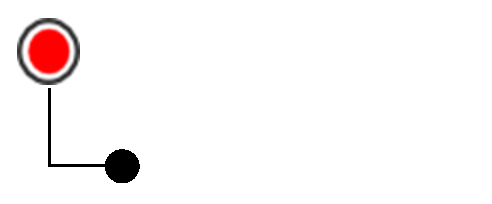
\includegraphics[scale=0.5]{img/kropki.eps}
	\end{center}
\end{wrapfigure}

\textbf{{\LARGE \nazwa}} \\
\linebreak
\textbf{ {\indent \indent \LARGE specification}}\\
\vskip 0.8 true in

\begin{figure}[htbp!]
	\centering
	\includegraphics[height=10cm]{img/SaymaT.jpg}\\
	%	\caption{v3.1(02.2017)}
\end{figure}
\begin{center}
	v1.0(11.2017)
\end{center}

\vskip 0.7 true in





\end{titlepage}

%\maketitle



\begin{table}[h!]
\vspace{5cm}
	\centering
	\begin{center}
\begin{tabular}{|l|l|}
	\hline
	\textbf{\rule[-2ex]{0pt}{5.5ex} Document version:} & Preliminary   \\ \hline
\textbf{\rule[-2ex]{0pt}{5.5ex} Issue Date:} & \today         \\ \hline
\textbf{\rule[-2ex]{0pt}{5.5ex} Written by:}      &  Filip Świtakowski                       \\ \hline
\textbf{\rule[-2ex]{0pt}{5.5ex} Approved by:}     &         Greg Kasprowicz      \\ \hline
	\textbf{\rule[-2ex]{0pt}{5.5ex} Document title:}  &  \nazwa - specification \\ \hline

\end{tabular} 
\end{center}
\end{table}

\clearpage


\listoftodos
\clearpage
\tableofcontents



\clearpage


\section{uTCA.4 Overview}

MicroTCA (uTCA) is Sinara's preferred form-factor for hardware with
high-speed data converters requiring deterministic phase control, such
as the \href{Sayma}{\emph{Sayma}} 2.4 GSPS smart arbitrary waveform
generator (SAWG).

uTCA is a modular, open standard originally developed by the
telecommunications industry. It allows a single rack master -- the Micro
TCA Carrier Hub (MCH) -- to control multiple slave boards, known as
Advanced Mezzanine Cards (AMCs) via a high-speed digital backplane. uTCA
chassis and backplanes are available commercially of the shelf (COTS).

We make use one of the most recent extension to the uTCA standard, uTCA.4.
Originating in the high-energy and particle physics (HEPP) community,
uTCA.4 introduces rear-transition modules (RTMs) along with a second
backplane for low-noise RF signals (RFBP). Each RTM connects to an AMC
(one RTM per AMC). Typically, the AMCs hold FPGAs and other high-speed
digital hardware, communicating with the MCH via gigabit serial links
over the AMC backplane. The RTMs hold data converters and other
low-noise analog components, controlled by the corresponding AMC. The
RFBP provides low-noise clocks and local oscillators (LOs). The RTMs and
RFBP are screened from the AMCs to minimise interference from the
high-speed digital logic.

\begin{figure}[htbp!]
\centering
\includegraphics[width=15cm]{img/MTCA_Front1.jpg}
\caption{Micro TCA chassis with 3 Sayma AMC modules inserted}
\end{figure}

\todo[inline]{New Figure: add photo of Sayma\_AMC attached to Sayma\_RTM sitting on bench so how they're connected is clear.}

(above) Micro TCA chassis with 3 Sayma AMC modules inserted.

Micro TCA chassis with 4 RTM modules inserted. One of them with 4
BaseMod AFE mezzanines installed.

\begin{figure}[htbp!]
\centering
\includegraphics[width=15cm]{img/MTCA_Back.jpg}
\caption{Micro TCA chassis with 4 RTM modules inserted. One of them has
4 BaseMod AFE mezzanines installed.}
\end{figure}


\href{http://www.nateurope.com/products/NAT-LLRF-Backplane.html}{RF
BP datasheet}



\section{uTCA parts and suppliers}\label{utca-parts-and-suppliers}

\begin{itemize}
\item NAT AC 600D, qty 1
\item NAT MCH-Basic v3.5, mid-size front panel, qty 1
\item NAT Native-R5, qty 1
\end{itemize}

\section{Schematic / Layout Viewer}\label{schematic-layout-viewer}


Hardware was designed under Mentor Graphics Xpedition Enterprise and Altium Designer CAD tools.
Project resources are in two separate folders:
\begin{itemize}
	\item ARTIQ\_EE folder is for designs made with the Mentor Graphics Xpedition Enterprise CAD tool.
	\item ARTIQ\_ALTIUM folder is for designs made with Altium Designer CAD tool.
\end{itemize}
Read-only access to PCB schematics and layout designs is possible using free tools.\\
Mentor has a free tool called
\href{https://www.mentor.com/pcb/downloads/visecad-viewer/}{visECAD
Viewer}.\\
Altium has a free tool called 
\href{http://www.altium.com/altium-designer-viewer}{Altium Designer viewer}

\clearpage

\section{Sayma}

Sayma is a hardware that supports M-Lab's Smart Arbitrary Waveform Generator(\href{http://m-labs.hk/artiq/manual-master/core_drivers_reference.html?highlight=sawg#module-artiq.coredevice.sawg}{SAWG}) gateware.
Provide 8 channels of
1.2 GSPS 16-bit DACs (2.4 GHz DAC clock) and 125 MSPS 16-bit ADCs. It
consists of an AMC, providing the high-speed digital logic, and a RTM,
holding the data converters and analog components.

The design files are located in
\href{https://github.com/m-labs/sinara/tree/master/ARTIQ_EE/PCB_Sayma_AMC}{ARTIQ\_EE/PCB\_Sayma\_AMC}
and
\href{https://github.com/m-labs/sinara/tree/master/ARTIQ_EE/PCB_Sayma_RTM}{ARTIQ\_EE/PCB\_Sayma\_RTM}
and, the AMC schematic is
\href{https://github.com/m-labs/sinara/blob/master/ARTIQ_EE/Sayma_AMC.pdf}{here}
and the RTM schematic is
\href{https://github.com/m-labs/sinara/blob/master/ARTIQ_EE/Sayma_RTM.pdf}{here}.
The PCBs are double width, mid height AMC module. Sayma AMC

\subsection{Features}\label{features}

\begin{itemize}

\item
  May be used in a uTCA rack or stand-alone operation with fibre-based
  DRTIO link
\item
  Analog input and output front-ends provided by plug-in
  \href{https://github.com/m-labs/sinara/wiki/SaymaAFE}{AFE} modules (eg BaseMod) for maximum
  flexibility.
\item
  Extremely flexible \href{https://github.com/m-labs/sinara/wiki/SinaraClocking}{clocking options}
\item
  Flexible feedback to SAWG parameters planned. Specification
  \href{https://github.com/m-labs/sinara/wiki/Servo}{here}.
\end{itemize}

\subsection{Key AMC Components}\label{key-amc-components}


\noindent

\textbf{Programmable resources:}

\begin{itemize}
	\item Xilinx Kintex UltraScale – XCKU040-1FFVA-1156C    FPGA 20 I/O, 530K
	Logic Cells
	\begin{itemize}
		\item speed grade: -1
		\item 20 GTH transceivers (Max Preformance 16.3 Gb/s)
	\end{itemize}
	\item MMC: LPC17762984
\end{itemize}	

\textbf{Memory:}

\begin{itemize}
	\item 512Mb  DDR3 SDRAM (32-bit interface), 800MHz (clock)
	\item 1Gb  DDR3 SDRAM (64-bit interface), 800MHz (clock)
	\item SPI Flash for FPGA configuration. Accessible by MMC
	\item SPI Flash for user data storage
	\item EEPROM with MAC and unique ID 
	
\end{itemize}

\textbf{Connectivity:}

\begin{itemize}
	\item 1 high pin count (HPC) FMC slot for single width mezzanine card
	\item Micro-USB UART connected to FPGA or MMC
	\item Stand-alone 12V power connector 
	\item MGT (Multi-Gigabit Transceiver) connected to:
	\begin{itemize}
		%		\item FMC x1
		\item RTM x16
		\item Fat\_Pipe1 x2
		%		\item AMC P2P x4
		%		\item Port 0 – possibility connected to SATA
		\item SFP x2
	\end{itemize}
	%	\item RTM connector with 8 GTP routed to it. Compatible with Sayma RTM module.
	\item  Port 0 – possibility connected to SATA
	\item RTM connector compatible with Sayma RTM module
	
\end{itemize}

\textbf{Supply:}

\begin{itemize}
	\item Monitoring of voltage and Power supply for RTM 12V and FMC 12V
	\item FMC VADJ fixed to 1V8
	\item Monitoring current of all FMC buses
	\item Stand-alone power connectore
	%	\item Czy Exar monitoruje powera? 
	
\end{itemize}


\textbf{Clocking:}

\begin{itemize}
	\item Clock recovery Si5324  is a precision clock multiplier andjitter attenuator
	\item UFL CLK input
	\item SMA CLK output
	
	
\end{itemize}


\textbf{Other:}

\begin{itemize}
	\item Temperature, voltage and current monitoring for critical power buses
	\item Temperature monitoring: FMC1, supply, FPGA core, DDR memory
	\item JTAG multiplexer (SCANSTA) for FMC access, local JTAG port and remote debug/Chipscope via Ethernet
	
\end{itemize}

\subsection{Key RTM Components}\label{key-rtm-components}
\todo[inline]{not sure if it should be here? only in RTM doc?}
\begin{itemize}

\item
  \textbf{DAC}: AD9154 4-channel high-speed data converter

  \begin{itemize}

  \item
    data rate is 1.2 GS/s at 16-bit
  \item
    clock is up to 2.4 GHz (1x, 2x, 4x and 8x interpolating modes)
  \item
    supports mix-mode to emphasize power in 3rd Nyquist Zone
  \item
    interface is 8-lane JESD204B (subclass 1)
  \item
    power consumption is 2.11 W
  \item
    each Sayma has 2 AD9154
  \end{itemize}
\item
  \textbf{ADC}: AD9656 is a 4-channel high-speed digitizer

  \begin{itemize}

  \item
    data rate is 125 MS/s at 16-bit
  \item
    clock is up to 125 MHz
  \item
    650 MHz analog bandwidth
  \item
    interface is 8-lane, 8 Gb/s per lane, JESD204B (subclass 1)
  \item
    each Sayma has 2 AD9656
  \end{itemize}
\item
  \textbf{clock generation}: (summarized \href{SinaraClocking}{here})

  \begin{itemize}

  \item
    Sayma has several distinct clock domains

    \begin{itemize}

    \item
      DAC, JESB204B output clock
    \item
      ADC, JESD204B input clock
    \item
      LO for analog mezzanines
    \end{itemize}
  \item
    These clocks may be generated using a low phase noise
    \href{ClockMezzanines}{Clock Mezzanine} PCB. A single Clock
    Mezzanine can be shared by several Sayma in a uTCA crate using
    {[}Baikal{]} PCB and an RTM RF backplane. Alternately, each Sayma
    can have its own distinct Clock Mezzanine (local generation).
  \end{itemize}
\item
  \textbf{clock distribution}

  \begin{itemize}

  \item
    HMC7043 SPI 14-Output Fanout Buffer for JESD204B
  \item
    HMC830 SPI fractional-N PLL
  \end{itemize}
\item
  \textbf{calibration ADC}: AD7194BCPZ is a 20-bit ADC for
  monitoring/calibration
\end{itemize}





\clearpage

%\section{Introduction to Micro TCA}




%The MTCA platform is available on the market for over
%ten years. It evolved from telecommunication ATCA standard. The MTCA sandard utilizes ATCA-defined AMC boards
%used directly in dedicated chassis. It also defines MTCA
%Carrier Hub (MCH) which controlls multiple slave boards, known as Advanced Mezzanine Cards (AMCs) via a high-speed digital backplane. AMC card can be equipped with FPGA Mzzanine Cards (FMCs) which are I/O modules pluggable to High-pin Count (HPC) or Low-pin Count (LPC) connector. 
%
%%which consists of Ethernet hub and crate
%%management system. 
%The MTCA crates are available in several
%form-factors for industrial, aviation and military use.
%User can easily extend and adopt the standard to particular application by selection of
%proper chassis, cooling method, computing and connectivity
%technology while keeping same mechanical, electrical standard and software architecture.\\


%MicroTCA (uTCA) is Sinara's preferred form-factor for hardware with high-speed data converters requiring deterministic phase control, such as the Sayma 2.4GSPS smart arbitrary waveform generator (SAWG).
%
%uTCA is a modular, open standard originally developed by the telecommunications industry. It allows a single rack master -- the Micro TCA Carrier Hub (MCH) -- to control multiple slave boards, known as Advanced Mezzanine Cards (AMCs) via a high-speed digital backplane. uTCA chassis and backplanes are available commercially of the shelf (COTS).
%%
%We make use of the most recent extension to the uTCA standard, uTCA.4. Originating in the high-energy and particle physics (HEPP) community, uTCA.4 introduces rear-transition modules (RTMs) along with a second backplane for low-noise RF signals (RFBP). Each RTM connects to an AMC (one RTM per AMC). Typically, the AMCs hold FPGAs and other high-speed digital hardware, communicating with the MCH via gigabit serial links over the AMC backplane. The RTMs hold data converters and other low-noise analog components, controlled by the corresponding AMC. The RFBP provides low-noise clocks and local oscillators (LOs). The RTMs and RFBP are screened from the AMCs to minimise interference from the high-speed digital logic

\section{Glossary}

\begin{description}
	\item[AMC Module or Modul] An AMC Module is a mezzanine or modular add-on card that extends the
	functionality of a Carrier Board. The term is also used to generically refer to the
	different varieties of Multi-Width and Multi-Height Modules.
	\item[Fat Pipes] Ports 4 though 11 of the AMC Connector constitute the Fat Pipes Region. This
	Region of Ports is intended for the assignment of multiple Lane interfaces, also
	called “fat pipes”. Fat Pipe 1 [Ports 4-7], Fat Pipe [Ports 8-11].
	\item[FMC] FPGA Mezzanine Card
	\item[Hot Swap] To remove a component (e.g., an AMC Module) from a system (e.g., an AMC Carrier
	AdvancedTCA Board) and plug in a new one while the power is still on and the
	system is still operating.
	\item[Management Power or MP] The 3.3V power for a Module's Management function, individually provided to each Slot by the Carrier
	\item[IPMB] ntelligent Platform Management Bus. The lowest level hardware management bus
	as described in the Intelligent Platform Management Bus Communications Protocol
	Specification.
	\item[MGT] Multi-Gigabit Transceiver
	\item[MMC] Module Management Controller. The MMC is the required intelligent controller that
	manages the Module and is interfaced to the Carrier via IPMB-Local
	\item[RTM] Rear Transition Module
\end{description}



\clearpage


%\section{Project description}
%	
%The Sayma RTM module extends Sayma AMC board connectivity by DACs and ADCs modules.
%
	

\section{Functional specifications}

\noindent

\textbf{Programmable resources:}

\begin{itemize}
\item Xilinx Artix-7 XC7A15T-1CSG325

\end{itemize}	

\textbf{Memory:}

\begin{itemize}

	\item EEPROM with MAC and unique ID 
	
\end{itemize}

\textbf{Connectivity:}

\begin{itemize}
	\item 4x mezzaninne connector LSS-120-01-L-DV-A 
	\item 40x SMP connector for ADC/DAC
%	\item Stand-alone 12V power connector 
	\item RTM connector with 16 GTP pair routed to it.
	\item GTP on RTM connector connected to:
	\begin{itemize}
		\item DAC x16 [Tx]
		\item ADC x8 [Rx]
		\item FPGA MGT 2x2 [Tx + Rx]
		\item SATA x2 
	\end{itemize}
	\item uRFB connector
	
\end{itemize}

\textbf{Supply:}

\begin{itemize}
	\item Monitoring of voltage and Power supply for FPGA and P3V3
	
\end{itemize}


\textbf{Clocking:}

\begin{itemize}
	\item UFL CLK input
	\item SMA CLK output
	\item Si5324 Clock recovery
	
\end{itemize}


\textbf{Other:}

\begin{itemize}
	\item Temperature, voltage and current monitoring for critical power buses

	
\end{itemize}









\clearpage


\section{Product view}	
	
	\begin{figure}[htbp!]
		\centering
		\includegraphics[width=17cm]{img/top1.jpg}\\
		\caption{Top view}
	\end{figure}
	
		\begin{figure}[htbp!]
			\centering
			\includegraphics[width=17cm]{img/bot1.jpg}\\
			\caption{Bottom view}
		\end{figure}

%		\begin{figure}[htbp!]
%			\centering
%			\includegraphics[width=17cm]{img/front.jpg}\\
%			\caption{Front view}
%		\end{figure}
%	

\clearpage

\section{Routing}


This section contain general blockm scheme of SAYMA AMC board and I2C map with addresses. General Block Scheme -figure \ref{BlockScheme}
shows more important connections between components. I2C connections with addresses can be found in figure \ref{I2C}. Detailed clocking scheme can be found in next paragraph in figure \ref{clocking}.
	\begin{figure}[htbp!]
		\centering
		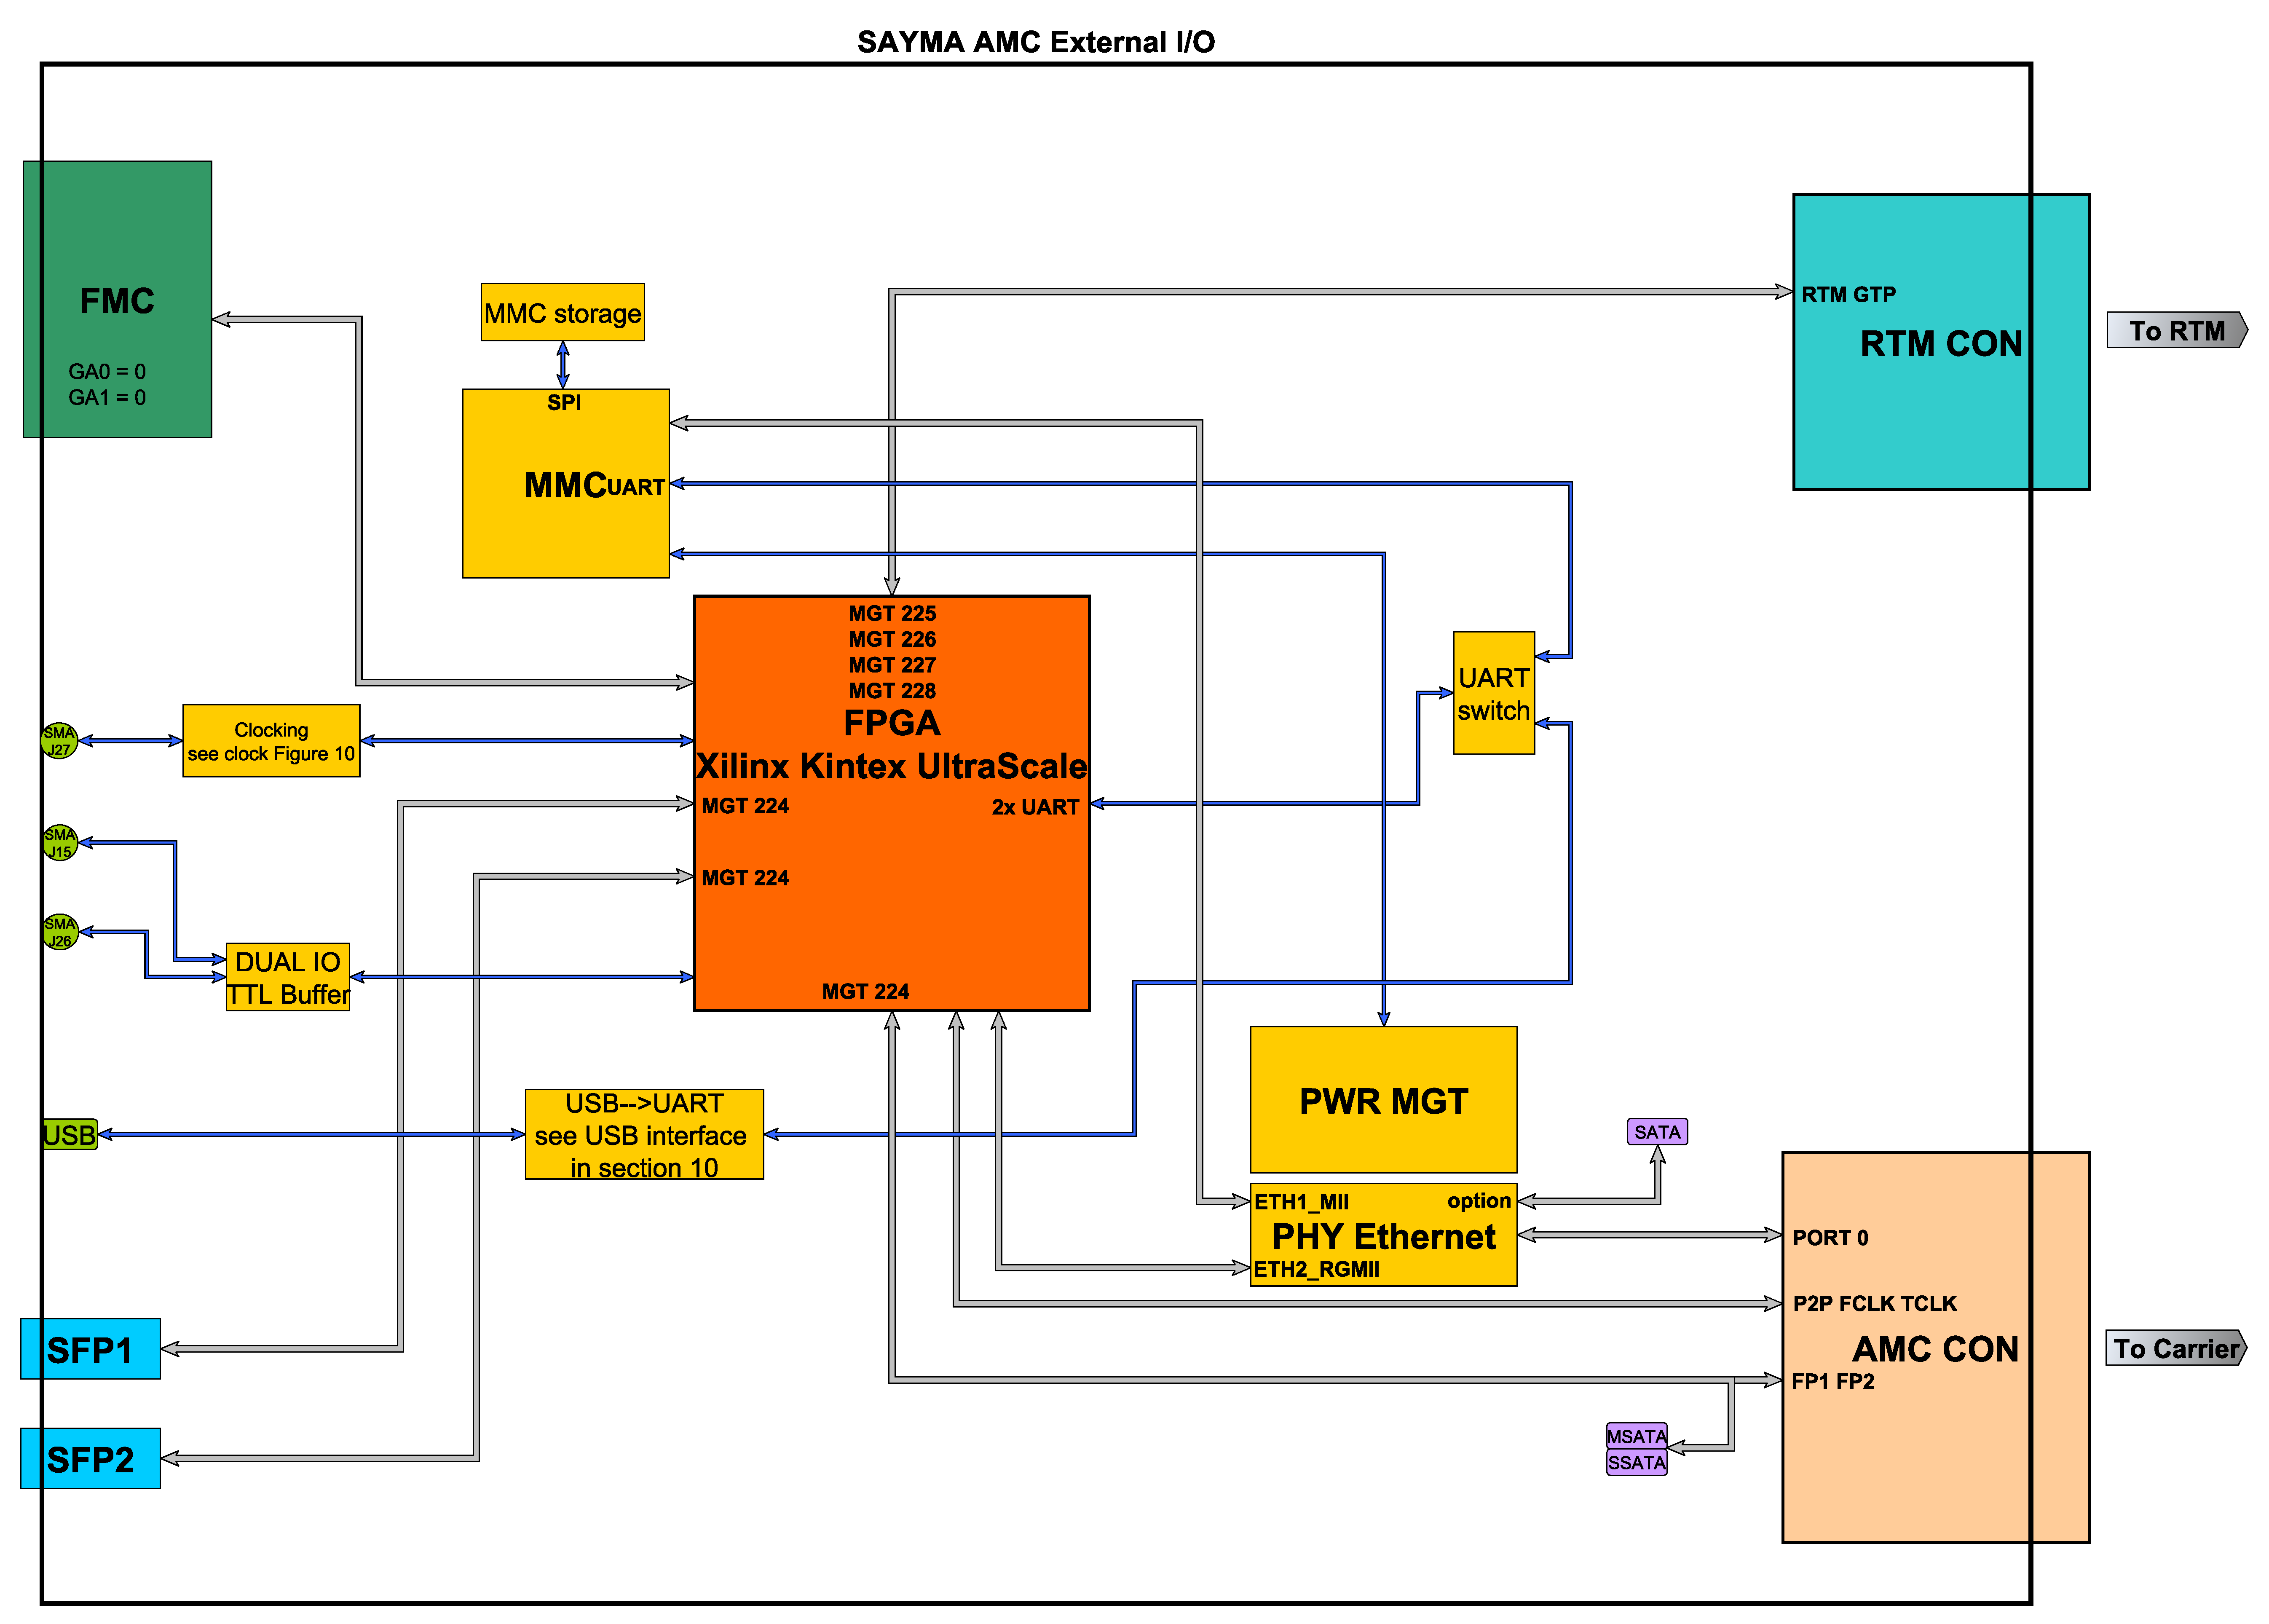
\includegraphics[scale=0.2]{img/sch.eps}\\
		\caption{General Block Scheme}\label{BlockScheme}
	\end{figure}

\clearpage5
	\begin{figure}[htbp!]
		\centering
		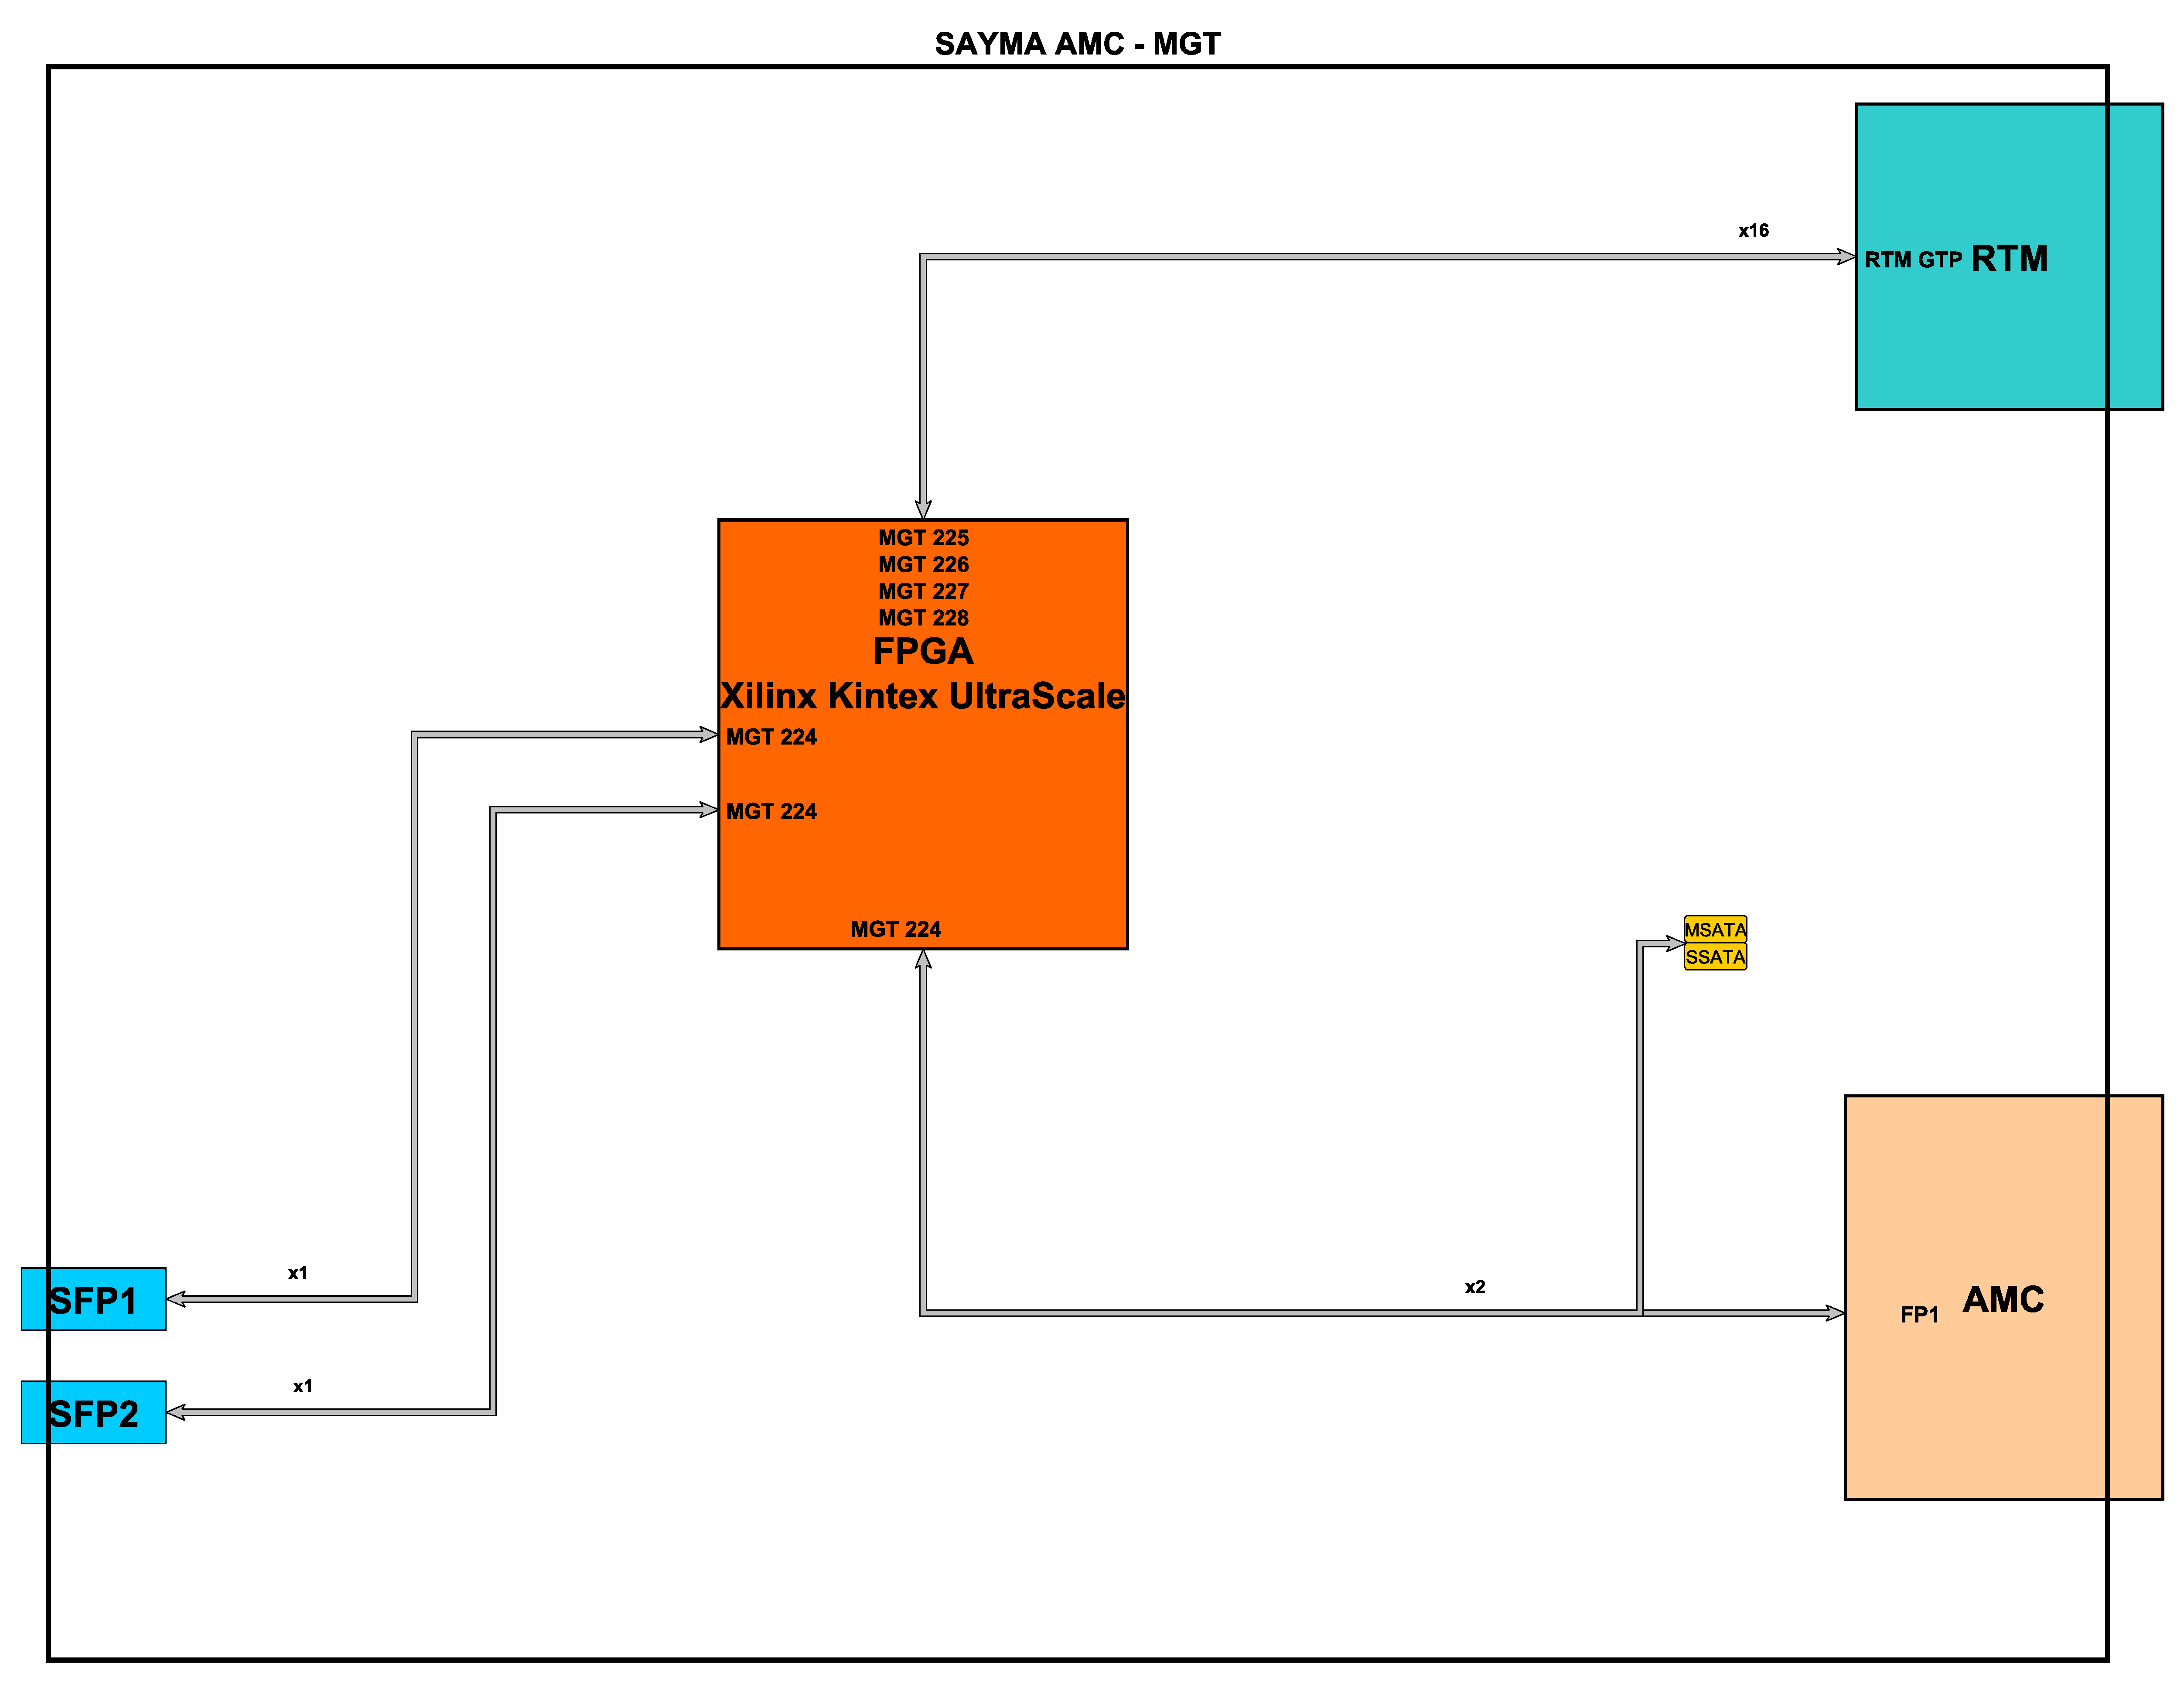
\includegraphics[scale=0.2]{img/sch_mgt.eps}\\
		\caption{MGT} \label{MGT}
	\end{figure}
	
\begin{longtable}{|c|c|c|}\hline
Transceiver MGT & Direction & Routed to \\ \hline
0\_224 & TX & SFP1 \\ \hline
0\_224 & RX & SFP1 \\ \hline
1\_224 & TX & SFP2 \\ \hline
1\_224 & RX & SFP2 \\ \hline
2\_224 & TX & FP1 or MASTER SATA \\ \hline
2\_224 & RX & FP1 or MASTER SATA\\ \hline
3\_224 & TX & FP1 or SLAVE SATA\\ \hline
3\_224 & RX & FP1 or SLAVE SATA\\ \hline
0\_225 & TX & RTM\_GTP \\ \hline
0\_225 & RX & RTM\_GTP \\ \hline
1\_225 & TX & RTM\_GTP \\ \hline
1\_225 & RX & RTM\_GTP \\ \hline
2\_225 & TX & RTM\_GTP \\ \hline
2\_225 & RX & RTM\_GTP \\ \hline
3\_225 & TX & RTM\_GTP \\ \hline
3\_225 & RX & RTM\_GTP \\ \hline
0\_226 & TX & RTM\_GTP \\ \hline
0\_226 & RX & RTM\_GTP \\ \hline
1\_226 & TX & RTM\_GTP \\ \hline
1\_226 & RX & RTM\_GTP \\ \hline
2\_226 & TX & RTM\_GTP \\ \hline
2\_226 & RX & RTM\_GTP \\ \hline
3\_226 & TX & RTM\_GTP \\ \hline
3\_226 & RX & RTM\_GTP \\ \hline
0\_227 & TX & RTM\_GTP \\ \hline
0\_227 & RX & RTM\_GTP \\ \hline
1\_227 & TX & RTM\_GTP \\ \hline
1\_227 & RX & RTM\_GTP \\ \hline
2\_227 & TX & RTM\_GTP \\ \hline
2\_227 & RX & RTM\_GTP \\ \hline
3\_227 & TX & RTM\_GTP \\ \hline
4\_227 & RX & RTM\_GTP \\ \hline
0\_228 & TX & RTM\_GTP \\ \hline
0\_228 & RX & RTM\_GTP \\ \hline
1\_228 & TX & RTM\_GTP \\ \hline
1\_228 & RX & RTM\_GTP \\ \hline
2\_228 & TX & RTM\_GTP \\ \hline
2\_228 & RX & RTM\_GTP \\ \hline
3\_228 & TX & RTM\_GTP \\ \hline
4\_228 & RX & RTM\_GTP \\ \hline
\end{longtable}	
	
	
\clearpage


The I2C MUX is made from two (TCA9548ARGER)  I2C multiplexers. In Sayma AMC there are two main I2C busses: MMC\_I2C and FPGA\_I2C. Each of them is connected to one multiplexer. Outputs are tied together, so Masters (MMC and FPGA) can acces to any of 7 I2C busses. Addidtionaly MMC has acces to FPGA\_I2C and is connected to IPMB through AMC connector.\\  
	\begin{figure}[htbp!]
		\centering
		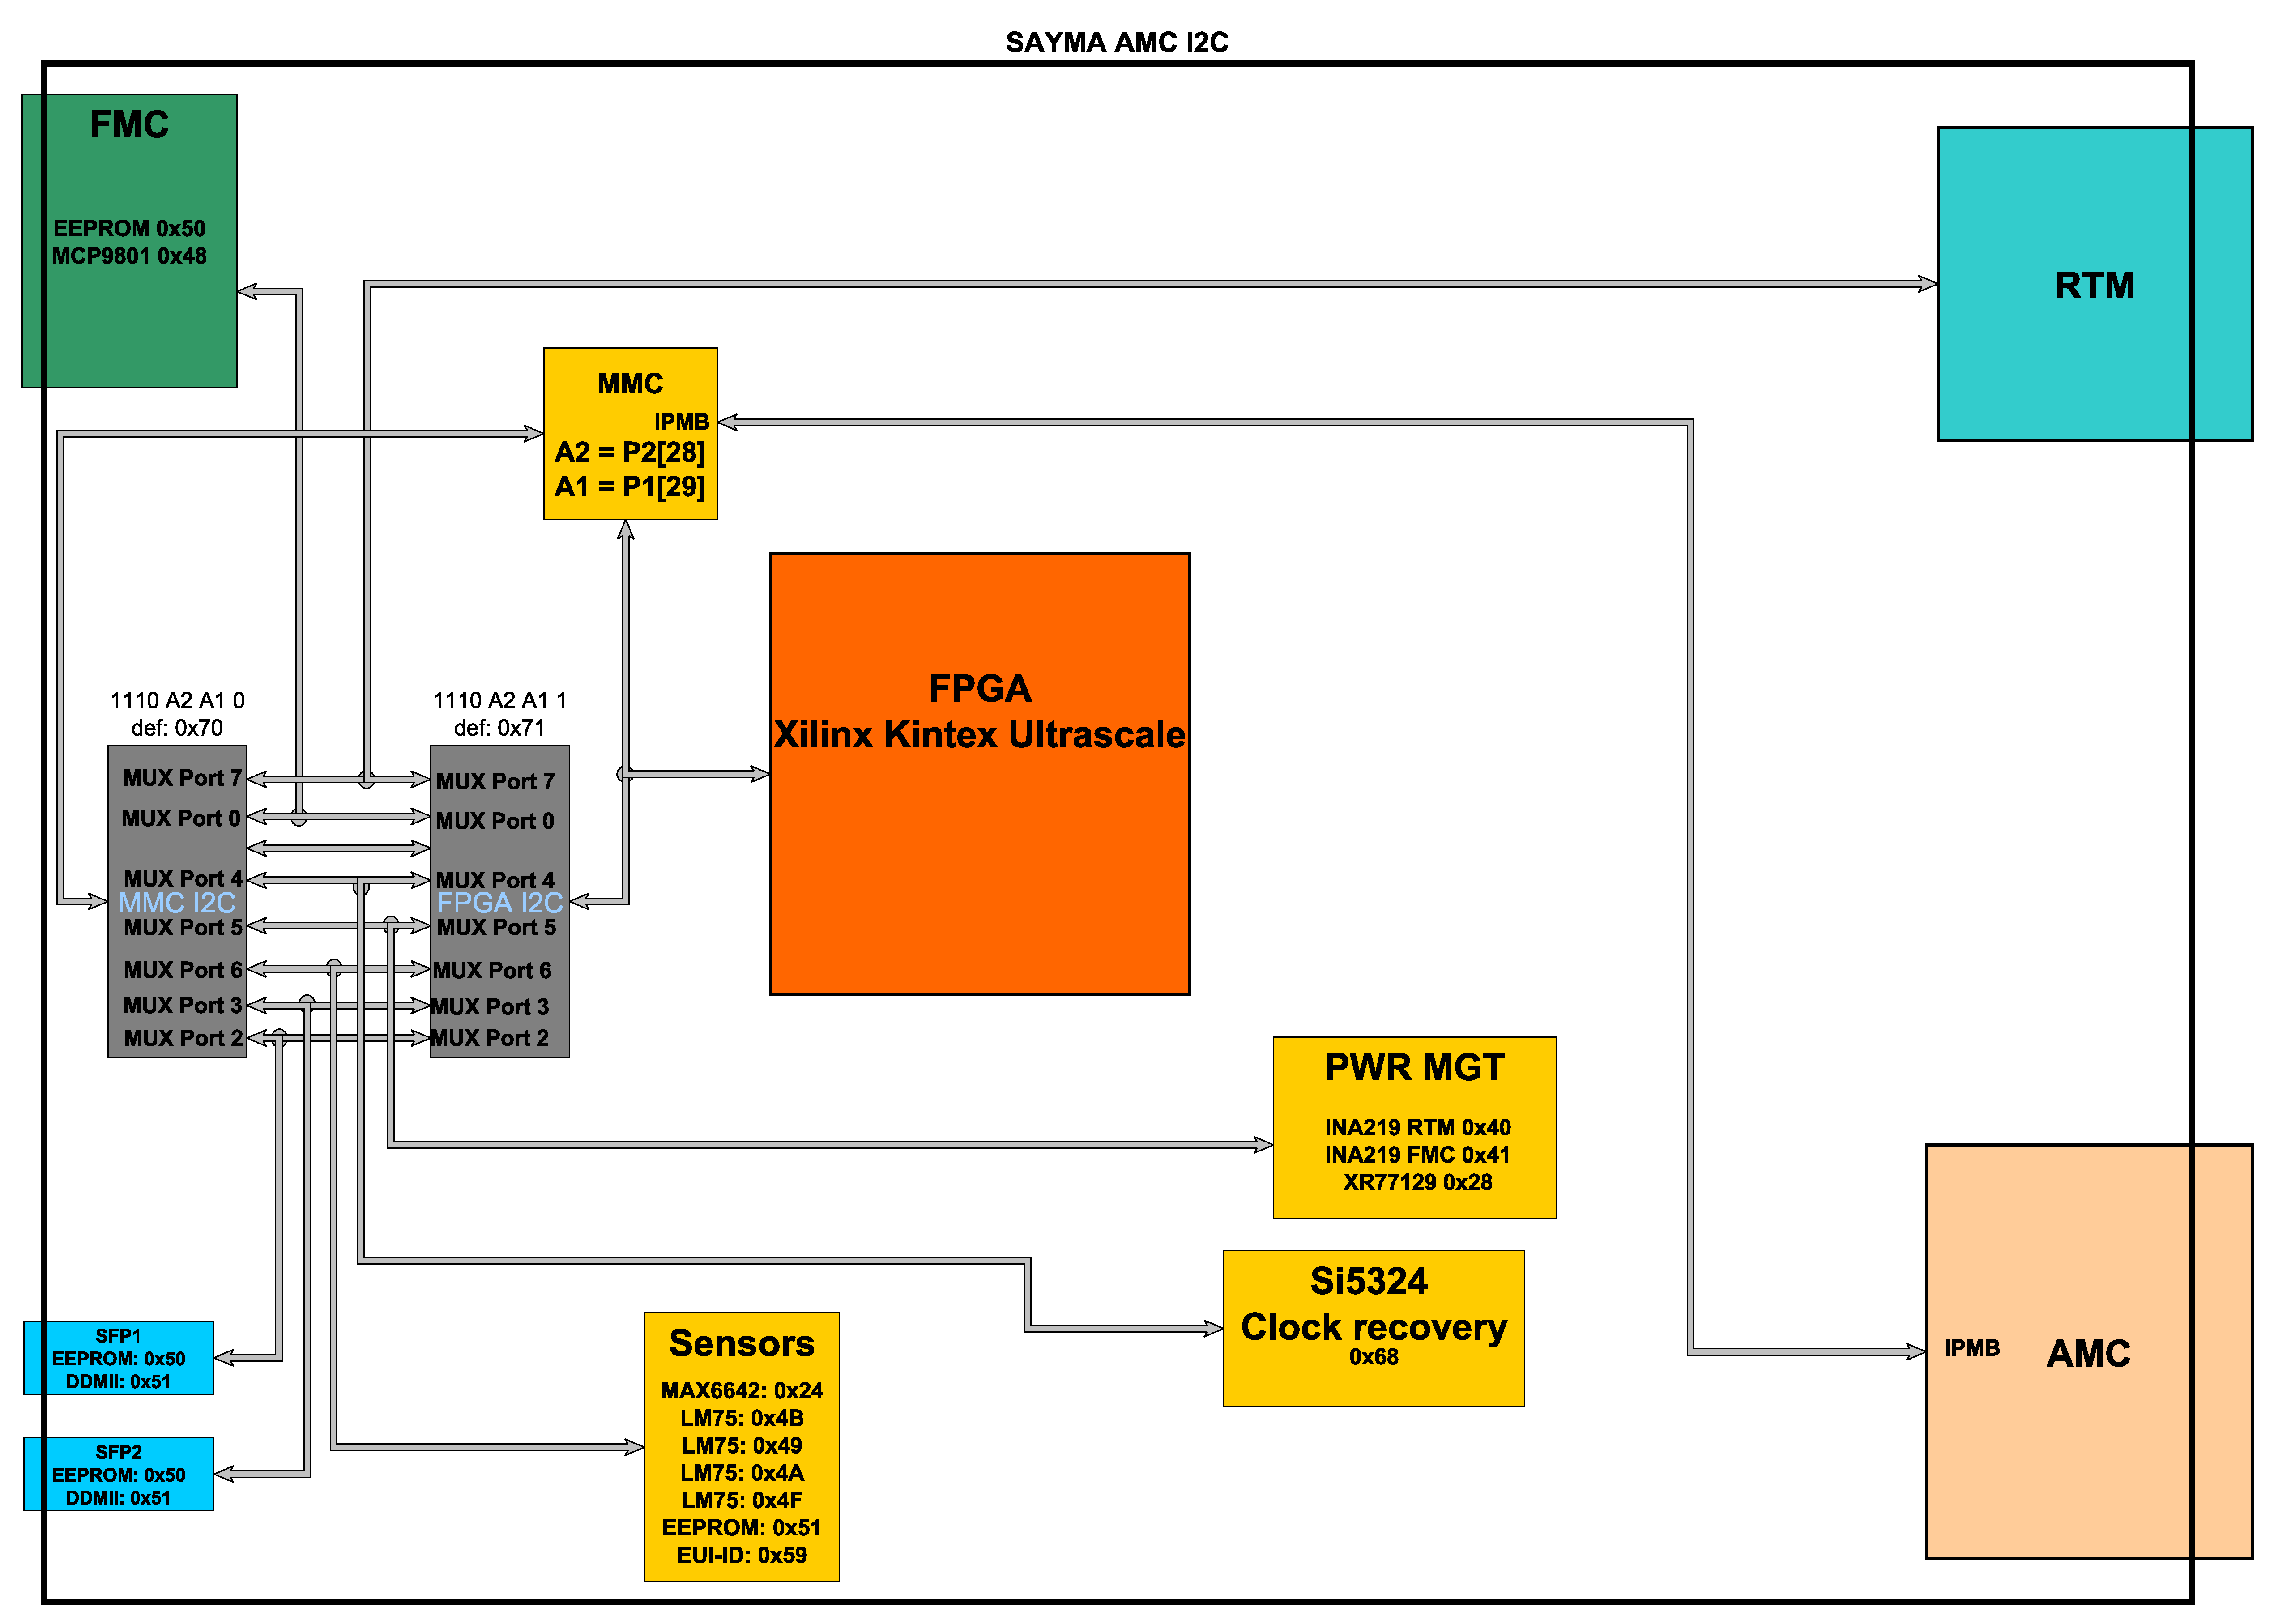
\includegraphics[scale=0.2]{img/i2c.eps}\\
		\caption{I2C map with addresses in hex} \label{I2C}
	\end{figure}


\clearpage

\section{Clocking}

This section describes how and where clock signals are routed.

	\begin{figure}[htbp!]
		\centering
		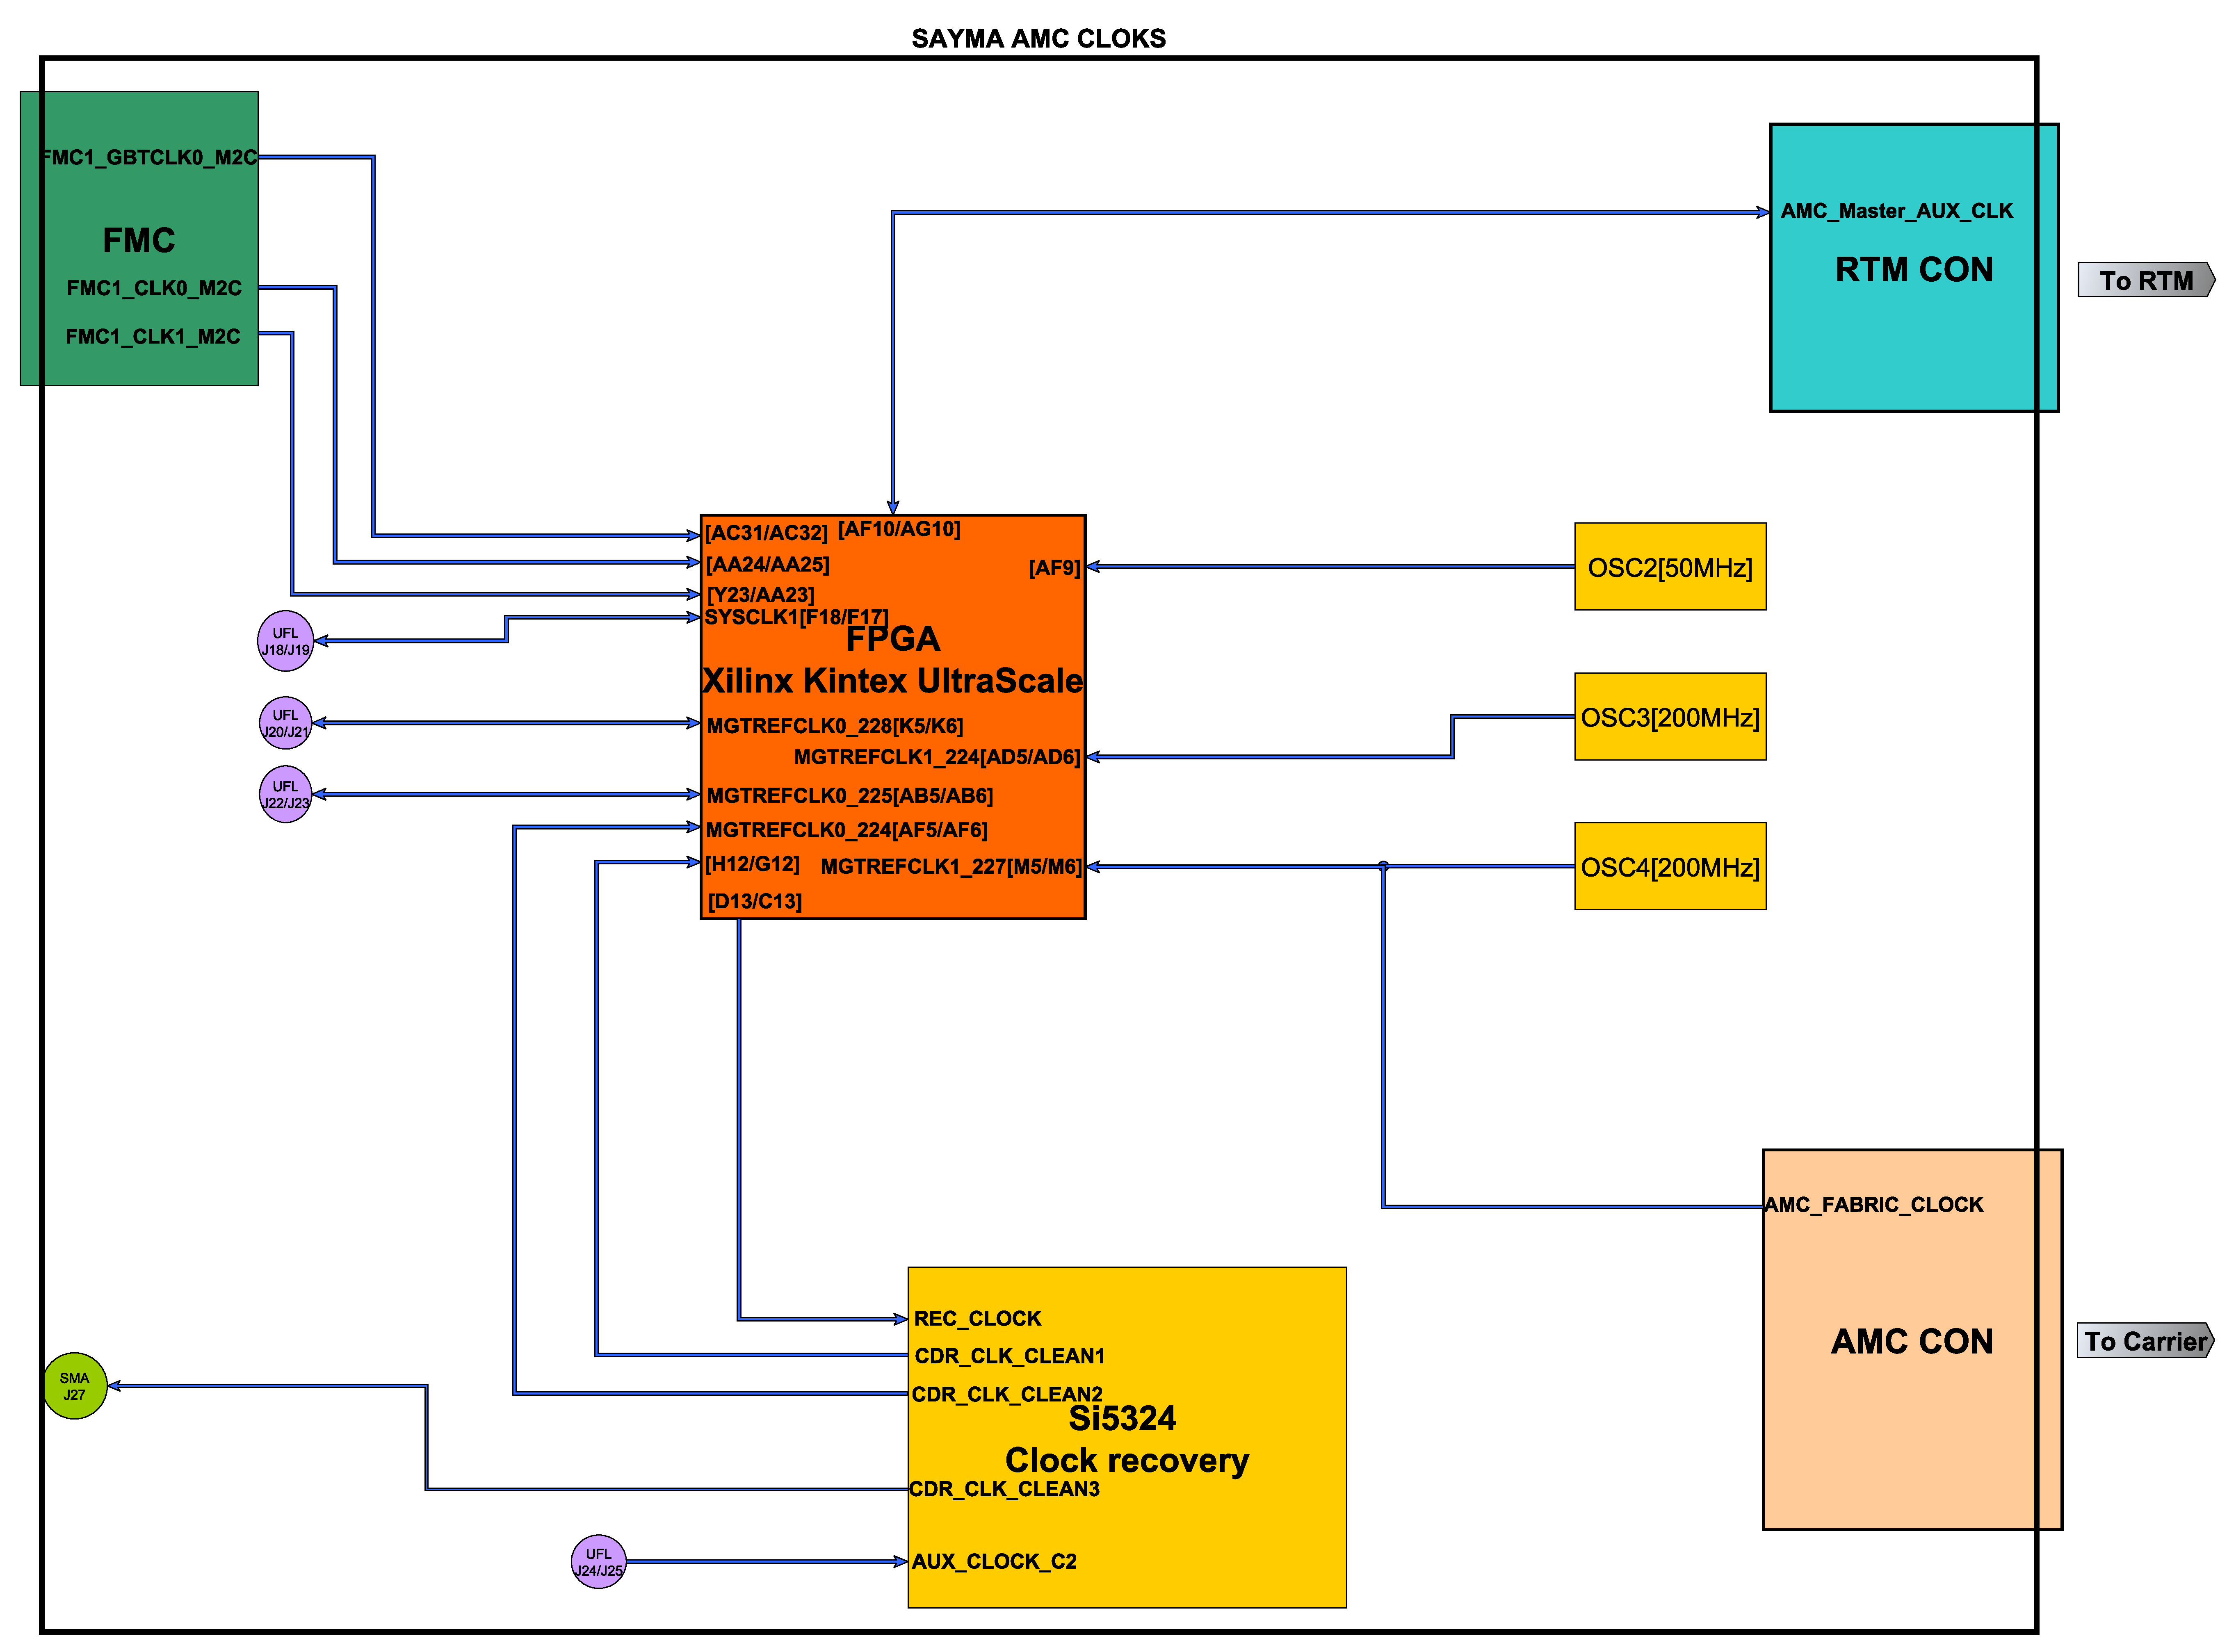
\includegraphics[scale=0.2]{img/clk.eps}\\
		\caption{Clocks} \label{clocking}
	\end{figure}
\begin{itemize}
	\item OSC2 - 50MHz main clock source for FPGA resources
	\item OSC3 - place-holder
	\item OSC4 dedicated 200MHz clock source to gigabit transceivers
\end{itemize}
\clearpage

\section{LEDs, ICs and headers}


		
		\begin{figure}[htbp!]
			\centering
			\includegraphics[width=12cm]{img/CalloutTop.png}\\
			\caption{Top view}
		\end{figure}
		
		\begin{figure}[htbp!]
			\centering
			\includegraphics[width=12cm]{img/CalloutBot.png}\\
			\caption{Bottom view}
		\end{figure}
\clearpage

\begin{longtable}{|c|c|c|} \hline
	\multicolumn{3}{|c|}{Call out table } \\ \hline	
	Call out & Designator & Description \\ \hline
	12 & J2 & RTM Connector \\ \hline
	13 & J74 & uRFB Connector \\ \hline
	14 & J76 & Mezzanine 1 Connector \\ \hline
	15 & J76 & Mezzanine 2 Connector \\ \hline
	16 & J76 & Mezzanine 3 Connector \\ \hline
	17 & J76 & Mezzanine 4 Connector \\ \hline	
	19 & J9 & CLK Mezzanine Connector\\ \hline
	20 & W1 & EXAR I2C header \\ \hline
	21 & J72 & Header with I/Os see Figure \ref{ios} \\ \hline
	22 & J70 & Master SATA  \\ \hline
	23 & J71 & Slave SATA \\ \hline
	24 & J73 & uRFB Conenctor \\ \hline
	25 & J4 & SMA, EXT 100 MHz input \\ \hline


\end{longtable}


Callout 18: U2 is
\begin{itemize}
	\item off if RTM is ok 
	\item red if RTM is in an error state
\end{itemize}

Callout 26: LD2 is
\begin{itemize}
	\item off if - user defined
	\item green if - user defined
\end{itemize}

Callout 27: LD1 is
\begin{itemize}
	\item off if RTM has initialized in crate
	\item blue if  power is cut off and is possible to remove the board
\end{itemize}

Callout 28: LD14 is
\begin{itemize}
	\item off if there is a problem with power converters
	\item green if all power chips send Power Good
\end{itemize}

Callout 25: LD15 is
\begin{itemize}
	\item off if RTM is ok
	\item green if RTM reach 80 degrees (power is cut off)
	\end{itemize}


\begin{longtable}{|c|c|c|c|c|c|c|} \hline
		\multicolumn{7}{|c|}{Power LED table }\\ \hline
	Call out & Designator & Description&  Colour &nominal state& IC &Failure\\ \hline
	1 & LD4 & P2V0 & Green & on & Power & off \\ \hline
	2 & LD9 & P12V0 & Green & on & Power & off \\ \hline 
	3 & LD8 & P1V8 & Green & on & Power & off \\ \hline 
	4 & LD7 & P1V2 & Green & on & Power & off \\ \hline 
	5 & LD6 & P1V0 & Green & on & Power & off \\ \hline 
	6 & LD16 & P12V0A & Green & on & Power & off \\ \hline 
	7 & LD10 & N12V0A & Green & on & Power & off \\ \hline 
	8 & LD17 & P3V3 & Green & on & Power & off \\ \hline 
	9 & LD3 & P4V0 & Green & on & Power & off \\ \hline 
	10 & LD5 & P6V0A & Green & on & Power & off \\ \hline  	
	11 & LD12 & N6V0A & Green & on & Power & off \\ \hline  		 
\end{longtable}

\subsection{Headers pinout}

		\begin{figure}[htbp!]
			\centering
			\includegraphics[width=8cm]{img/io.png}\\
			\caption{DIO - Call out 21} \label{ios}
		\end{figure}
%
%		\begin{figure}[htbp!]
%			\centering
%			\includegraphics[width=9cm]{img/jtaglpc.png}\\
%			\caption{JTAG - Call out  21}
%		\end{figure}
%		
%		\begin{figure}[htbp!]
%			\centering
%			\includegraphics[width=9cm]{img/gpio.png}\\
%			\caption{DIO - Call out 23}
%		\end{figure}

\clearpage


%\begin{longtable}{|c|c|c|} \hline
%		\multicolumn{3}{|c|}{Tespoints table}\\ \hline
%	TPx & Sig Name & LPC pin \\ \hline
%	TP1 & MII1\_col & C13 \\ \hline
%	TP2 & SDCLK & J10 \\ \hline
%	TP3 & SDCMD & K14 \\ \hline
%	TP4 & SDPWR & K11 \\ \hline
%	TP5 & SDDAT0 & L14 \\ \hline
%	TP6 & SDDAT1 & M12 \\ \hline
%	TP7 & SDDAT2 & N14 \\ \hline
%	TP8 & SDDAT3 & M11 \\ \hline
%	
%\end{longtable}	


\subsection{Location ICs}

		\begin{figure}[htbp!]
			\centering
			\includegraphics[width=12cm]{img/TU1.png}\\
			\caption{Top}
		\end{figure}
		\begin{figure}[htbp!]
			\centering
			\includegraphics[width=12cm]{img/BU1.png}\\
			\caption{Bottom}
		\end{figure}
\clearpage

\begin{longtable}{|c|c|c|} \hline
		\multicolumn{3}{|c|}{ICs Location}\\ \hline	
	Ux & IC & Description \\ \hline
	U1 & Artix-7 & FPGA \\ \hline
	IC1/IC43	&	TCA9548		& I2C MUX 			\\	\hline	
	IC3 & AD9154 & DAC1 \\ \hline
	IC4 & AD9154  & DAC2\\ \hline
	IC5/IC6/IC7	&	LT3045		&  	DAC supply		\\	\hline
	IC8/IC9/IC10/IC11	&	LT3045		&  	DAC supply		\\	\hline	
	IC12/IC13/IC14 & LT3045 & DAC supply \\ \hline
	IC15/IC16/IC17/IC18 & LT3045 & DAC supply \\ \hline	
	IC20	&	LT3045		&  DAC supply			\\	\hline	
	IC21	&	AD9656		&  	ADC		\\	\hline
	IC22 & AD9656 & ADC \\ \hline
	IC29 & ADP1740 & P1V8 LDO \\ \hline	
	IC32 &	LT3045 & Si5324 power supply \\ \hline
	IC33 & ADM7151 & P5V0 LDO \\ \hline
	IC36	&	AD7194		& ADC 			\\	\hline
	IC37	&	ADR440		&  ADC reference			\\	\hline
	IC38 & Si5324 & Clock recovery \\ \hline	
	IC39 & LM75 & Temp sens \\ \hline
	IC40 & LM75 & Temp sens \\ \hline	
	IC42 & PCF8574 & I2C to GPIO extender \\ \hline	
	IC44 & MAX6642 & Temp sens \\ \hline
	IC45	&	ADCLK948		&  Clock buffer		\\	\hline
	IC46	&	ADCLK948		& Clock buffer 		\\	\hline					
	IC47 & LTM4619 & Buck converter P2V0 and P4V0\\ \hline
	IC48 & TPS 74401  & Buck converter P6V0\\ \hline
	IC50 &  LTM8049 & Buck converter P12V0A and N12V0A \\ \hline
	IC51 & LTM8049& Buck converter N6V0A \\ \hline
	IC52 & ADCLK948 & Clock buffer \\ \hline
	IC54 &ADCLK948 & Clock buffer \\ \hline	
	IC53	&	LTC6957		&  Isolation external clock input			\\	\hline	
	IC55	&	LT3045		&  DAC supply			\\	\hline	
	IC56 & ADT7420 & Temp sens \\ \hline
	IC57 & ADT7420 & Temp sens \\ \hline
	IC58	&	HMC7043		&  	Clock buffer		\\ \hline
	IC59	&	HMC830		&  	Clock buffer		\\	\hline
	IC62/IC63		& LT3045	& HMC7043 power supply	\\ \hline			
	IC64 & XR77129 & EXAR \\ \hline
	IC66 & AT24MAC402 & EEPROM \\ \hline
	T4/T8/T9/T10 & FDMS7608S & Exar transistors\\ \hline




																										
\end{longtable}




\clearpage

\section{FMC}



\begin{itemize}
	\item VADJ: 1V8 @ 1A
	\item FPGA Banks: 47HP and 48HP
\end{itemize}


The connector is compliant with ANSI/VITA 57.1 FMC-LPC Standard.\\

%---------------------------------------------------------FMC1
\begin{footnotesize}
	\begin{longtable}{|p{7cm}|p{1cm}|p{5cm}|}
		\hline
		\multicolumn{3}{|c|}{\multirow{2}{*}{\textbf{\large{FMC1}}}}\\
		\multicolumn{3}{|c|}{} \\ \hline 
		FPGA signal	&	FPGA ball	&	Signal on the board	\\ \hline
		IO\_L12P\_T1U\_N10\_GC\_47	&	AA24	&	FMC1\_CLK0\_M2C\_P	\\ \hline
		IO\_L12N\_T1U\_N11\_GC\_47	&	AA25	&	FMC1\_CLK0\_M2C\_N	\\ \hline
		IO\_L11P\_T1U\_N8\_GC\_47	&	Y23	&	FMC1\_CLK1\_M2C\_P	\\ \hline
		IO\_L11N\_T1U\_N9\_GC\_47	&	AA23	&	FMC1\_CLK1\_M2C\_N	\\ \hline
		IO\_L12P\_T1U\_N10\_GC\_48	&	AC31	&	FMC1\_GBTCLK0\_M2C\_P	\\ \hline
		IO\_L12N\_T1U\_N11\_GC\_48	&	AC32	&	FMC1\_GBTCLK0\_M2C\_N	\\ \hline
		IO\_L1P\_T0L\_N0\_DBC\_48	&	AE27	&	FMC1\_DP0\_M2C\_P	\\ \hline
		IO\_L1N\_T0L\_N1\_DBC\_48	&	AF27	&	FMC1\_DP0\_M2C\_N	\\ \hline
		IO\_L2P\_T0L\_N2\_48	&	AE28	&	FMC1\_DP0\_C2M\_P	\\ \hline
		IO\_L2N\_T0L\_N3\_48	&	AF28	&	FMC1\_DP0\_C2M\_N	\\ \hline
		IO\_L13P\_T2L\_N0\_GC\_QBC\_48	&	AA32	&	FMC1\_LA00\_CC\_P	\\ \hline
		IO\_L13N\_T2L\_N1\_GC\_QBC\_48	&	AB32	&	FMC1\_LA00\_CC\_N	\\ \hline
		IO\_L14P\_T2L\_N2\_GC\_48	&	AB30	&	FMC1\_LA01\_CC\_P	\\ \hline
		IO\_L14N\_T2L\_N3\_GC\_48	&	AB31	&	FMC1\_LA01\_CC\_N	\\ \hline
		IO\_L8P\_T1L\_N2\_AD5P\_48	&	AF33	&	FMC1\_LA02\_P	\\ \hline
		IO\_L8N\_T1L\_N3\_AD5N\_48	&	AG34	&	FMC1\_LA02\_N	\\ \hline
		IO\_L21P\_T3L\_N4\_AD8P\_48	&	V33	&	FMC1\_LA03\_P	\\ \hline
		IO\_L21N\_T3L\_N5\_AD8N\_48	&	W34	&	FMC1\_LA03\_N	\\ \hline
		IO\_L7P\_T1L\_N0\_QBC\_AD13P\_48	&	AG31	&	FMC1\_LA04\_P	\\ \hline
		IO\_L7N\_T1L\_N1\_QBC\_AD13N\_48	&	AG32	&	FMC1\_LA04\_N	\\ \hline
		IO\_L10P\_T1U\_N6\_QBC\_AD4P\_48	&	AE33	&	FMC1\_LA05\_P	\\ \hline
		IO\_L10N\_T1U\_N7\_QBC\_AD4N\_48	&	AF34	&	FMC1\_LA05\_N	\\ \hline
		IO\_L15P\_T2L\_N4\_AD11P\_48	&	AC34	&	FMC1\_LA06\_P	\\ \hline
		IO\_L15N\_T2L\_N5\_AD11N\_48	&	AD34	&	FMC1\_LA06\_N	\\ \hline
		IO\_L18P\_T2U\_N10\_AD2P\_48	&	AC33	&	FMC1\_LA07\_P	\\ \hline
		IO\_L18N\_T2U\_N11\_AD2N\_48	&	AD33	&	FMC1\_LA07\_N	\\ \hline
		IO\_L11P\_T1U\_N8\_GC\_48	&	AD30	&	FMC1\_LA08\_P	\\ \hline
		IO\_L11N\_T1U\_N9\_GC\_48	&	AD31	&	FMC1\_LA08\_N	\\ \hline
		IO\_L9P\_T1L\_N4\_AD12P\_48	&	AE32	&	FMC1\_LA09\_P	\\ \hline
		IO\_L9N\_T1L\_N5\_AD12N\_48	&	AF32	&	FMC1\_LA09\_N	\\ \hline
		IO\_L17P\_T2U\_N8\_AD10P\_48	&	AA34	&	FMC1\_LA10\_P	\\ \hline
		IO\_L17N\_T2U\_N9\_AD10N\_48	&	AB34	&	FMC1\_LA10\_N	\\ \hline
		IO\_L16P\_T2U\_N6\_QBC\_AD3P\_48	&	AA29	&	FMC1\_LA11\_P	\\ \hline
		IO\_L16N\_T2U\_N7\_QBC\_AD3N\_48	&	AB29	&	FMC1\_LA11\_N	\\ \hline
		IO\_L24P\_T3U\_N10\_48	&	V31	&	FMC1\_LA12\_P	\\ \hline
		IO\_L24N\_T3U\_N11\_48	&	W31	&	FMC1\_LA12\_N	\\ \hline
		IO\_L19P\_T3L\_N0\_DBC\_AD9P\_48	&	W33	&	FMC1\_LA13\_P	\\ \hline
		IO\_L19N\_T3L\_N1\_DBC\_AD9N\_48	&	Y33	&	FMC1\_LA13\_N	\\ \hline
		IO\_L23P\_T3U\_N8\_48	&	U34	&	FMC1\_LA14\_P	\\ \hline
		IO\_L23N\_T3U\_N9\_48	&	V34	&	FMC1\_LA14\_N	\\ \hline
		IO\_L22P\_T3U\_N6\_DBC\_AD0P\_48	&	Y31	&	FMC1\_LA15\_P	\\ \hline
		IO\_L22N\_T3U\_N7\_DBC\_AD0N\_48	&	Y32	&	FMC1\_LA15\_N	\\ \hline
		IO\_L20P\_T3L\_N2\_AD1P\_48	&	W30	&	FMC1\_LA16\_P	\\ \hline
		IO\_L20N\_T3L\_N3\_AD1N\_48	&	Y30	&	FMC1\_LA16\_N	\\ \hline
		IO\_L13P\_T2L\_N0\_GC\_QBC\_47	&	W23	&	FMC1\_LA17\_CC\_P	\\ \hline
		IO\_L13N\_T2L\_N1\_GC\_QBC\_47	&	W24	&	FMC1\_LA17\_CC\_N	\\ \hline
		IO\_L14P\_T2L\_N2\_GC\_47	&	W25	&	FMC1\_LA18\_CC\_P	\\ \hline
		IO\_L14N\_T2L\_N3\_GC\_47	&	Y25	&	FMC1\_LA18\_CC\_N	\\ \hline
		IO\_L16P\_T2U\_N6\_QBC\_AD3P\_47	&	V22	&	FMC1\_LA19\_P	\\ \hline
		IO\_L16N\_T2U\_N7\_QBC\_AD3N\_47	&	V23	&	FMC1\_LA19\_N	\\ \hline
		IO\_L17P\_T2U\_N8\_AD10P\_47	&	T22	&	FMC1\_LA20\_P	\\ \hline
		IO\_L17N\_T2U\_N9\_AD10N\_47	&	T23	&	FMC1\_LA20\_N	\\ \hline
		IO\_L18P\_T2U\_N10\_AD2P\_47	&	V21	&	FMC1\_LA21\_P	\\ \hline
		IO\_L18N\_T2U\_N11\_AD2N\_47	&	W21	&	FMC1\_LA21\_N	\\ \hline
		IO\_L15P\_T2L\_N4\_AD11P\_47	&	U21	&	FMC1\_LA22\_P	\\ \hline
		IO\_L15N\_T2L\_N5\_AD11N\_47	&	U22	&	FMC1\_LA22\_N	\\ \hline
		IO\_L10P\_T1U\_N6\_QBC\_AD4P\_47	&	AB21	&	FMC1\_LA23\_P	\\ \hline
		IO\_L10N\_T1U\_N7\_QBC\_AD4N\_47	&	AC21	&	FMC1\_LA23\_N	\\ \hline
		IO\_L8P\_T1L\_N2\_AD5P\_47	&	AC22	&	FMC1\_LA24\_P	\\ \hline
		IO\_L8N\_T1L\_N3\_AD5N\_47	&	AC23	&	FMC1\_LA24\_N	\\ \hline
		IO\_L9P\_T1L\_N4\_AD12P\_47	&	AA20	&	FMC1\_LA25\_P	\\ \hline
		IO\_L9N\_T1L\_N5\_AD12N\_47	&	AB20	&	FMC1\_LA25\_N	\\ \hline
		IO\_L7P\_T1L\_N0\_QBC\_AD13P\_47	&	AA22	&	FMC1\_LA26\_P	\\ \hline
		IO\_L7N\_T1L\_N1\_QBC\_AD13N\_47	&	AB22	&	FMC1\_LA26\_N	\\ \hline
		IO\_L6P\_T0U\_N10\_AD6P\_47	&	AB25	&	FMC1\_LA27\_P	\\ \hline
		IO\_L6N\_T0U\_N11\_AD6N\_47	&	AB26	&	FMC1\_LA27\_N	\\ \hline
		IO\_L24P\_T3U\_N10\_47	&	V26	&	FMC1\_LA28\_P	\\ \hline
		IO\_L24N\_T3U\_N11\_47	&	W26	&	FMC1\_LA28\_N	\\ \hline
		IO\_L23P\_T3U\_N8\_47	&	V29	&	FMC1\_LA29\_P	\\ \hline
		IO\_L23N\_T3U\_N9\_47	&	W29	&	FMC1\_LA29\_N	\\ \hline
		IO\_L22P\_T3U\_N6\_DBC\_AD0P\_47	&	U26	&	FMC1\_LA30\_P	\\ \hline
		IO\_L22N\_T3U\_N7\_DBC\_AD0N\_47	&	U27	&	FMC1\_LA30\_N	\\ \hline
		IO\_L21P\_T3L\_N4\_AD8P\_47	&	W28	&	FMC1\_LA31\_P	\\ \hline
		IO\_L21N\_T3L\_N5\_AD8N\_47	&	Y28	&	FMC1\_LA31\_N	\\ \hline
		IO\_L20P\_T3L\_N2\_AD1P\_47	&	U24	&	FMC1\_LA32\_P	\\ \hline
		IO\_L20N\_T3L\_N3\_AD1N\_47	&	U25	&	FMC1\_LA32\_N	\\ \hline
		IO\_L19P\_T3L\_N0\_DBC\_AD9P\_47	&	V27	&	FMC1\_LA33\_P	\\ \hline
		IO\_L19N\_T3L\_N1\_DBC\_AD9N\_47	&	V28	&	FMC1\_LA33\_N	\\ \hline
		VREF\_48	&	AA30	&	FMC1\_VREF\_A\_M2C	\\ \hline
		VREF\_47	&	V24	&	FMC1\_VREF\_A\_M2C	\\ \hline
		
	\end{longtable}
\end{footnotesize}
\clearpage

\section{USB-UART}
\subsection{UART Switch}

UART from FPGA is connected through Multiplexer (SN74CB3T3257PW). Selection between MMC and USB is preformes automaticly. When micro-USB is connected S siglnal is high and Multiplexer connects USB to FPGA.\\ 

\subsection{USB-UART bridge}

The USB-UART bridge (FT4232H) requires USB device drivers, vailable free from http://www.ftdichip.com,
which are used to make the FT4232H on the Mini Module appear as a four virtual COM ports (VCP). This
then allows the user to communicate with the USB interface via a standard PC serial emulation port
(TTY).\\ Another FTDI USB driver, the D2XX driver, can also be used with application software to directly
access the FT4232H on the Mini Module though a DLL. \\


\clearpage

\section{JTAG}
Scansta112 is 7-Port Multidrop JTAG Multiplexer. It is used to partition scan chains into managable sizes, or to isolate specific devices onto a separate chain. By default Scansta input signal is from IDC header. AMC JTAG is connected to Master Port on SCANSTA, so it can be used as Master or Slave module. The rest modules (MMC, FPGA, FMC, RTM) are tied to slave SCANSTA outputs. \\

Tere are two JTAG sources – either AMC connector ( JSM module) or USB to JTAG bridge (FTDI chip). There is also onboard JTAG connector (Xilinx type) -J3. Insertion of JTAG programmer probe deactivates the FTDI JTAG connectivity and forces SCANSTA chip set this port as master port. By default SCANSTA selects AMC port as master one.\\


In Sayma AMC, SCANSTA112 is used in Transparent Sticher Mode. In this mode, the IC can be configured via hardware to skip the addressing protocol needed, sothere is no need to run a SVF configuration file on IMPACT when programming the FPGA bitstream.\\
	\begin{figure}[htbp!]
		\centering
		\includegraphics[scale=0.5]{img/jtag.png}\\
		\caption{USB-->JTAG} 
	\end{figure}
\clearpage	
General block scheme of Scansta connections is shown below.\\
	
		\begin{figure}[htbp!]
			\centering
			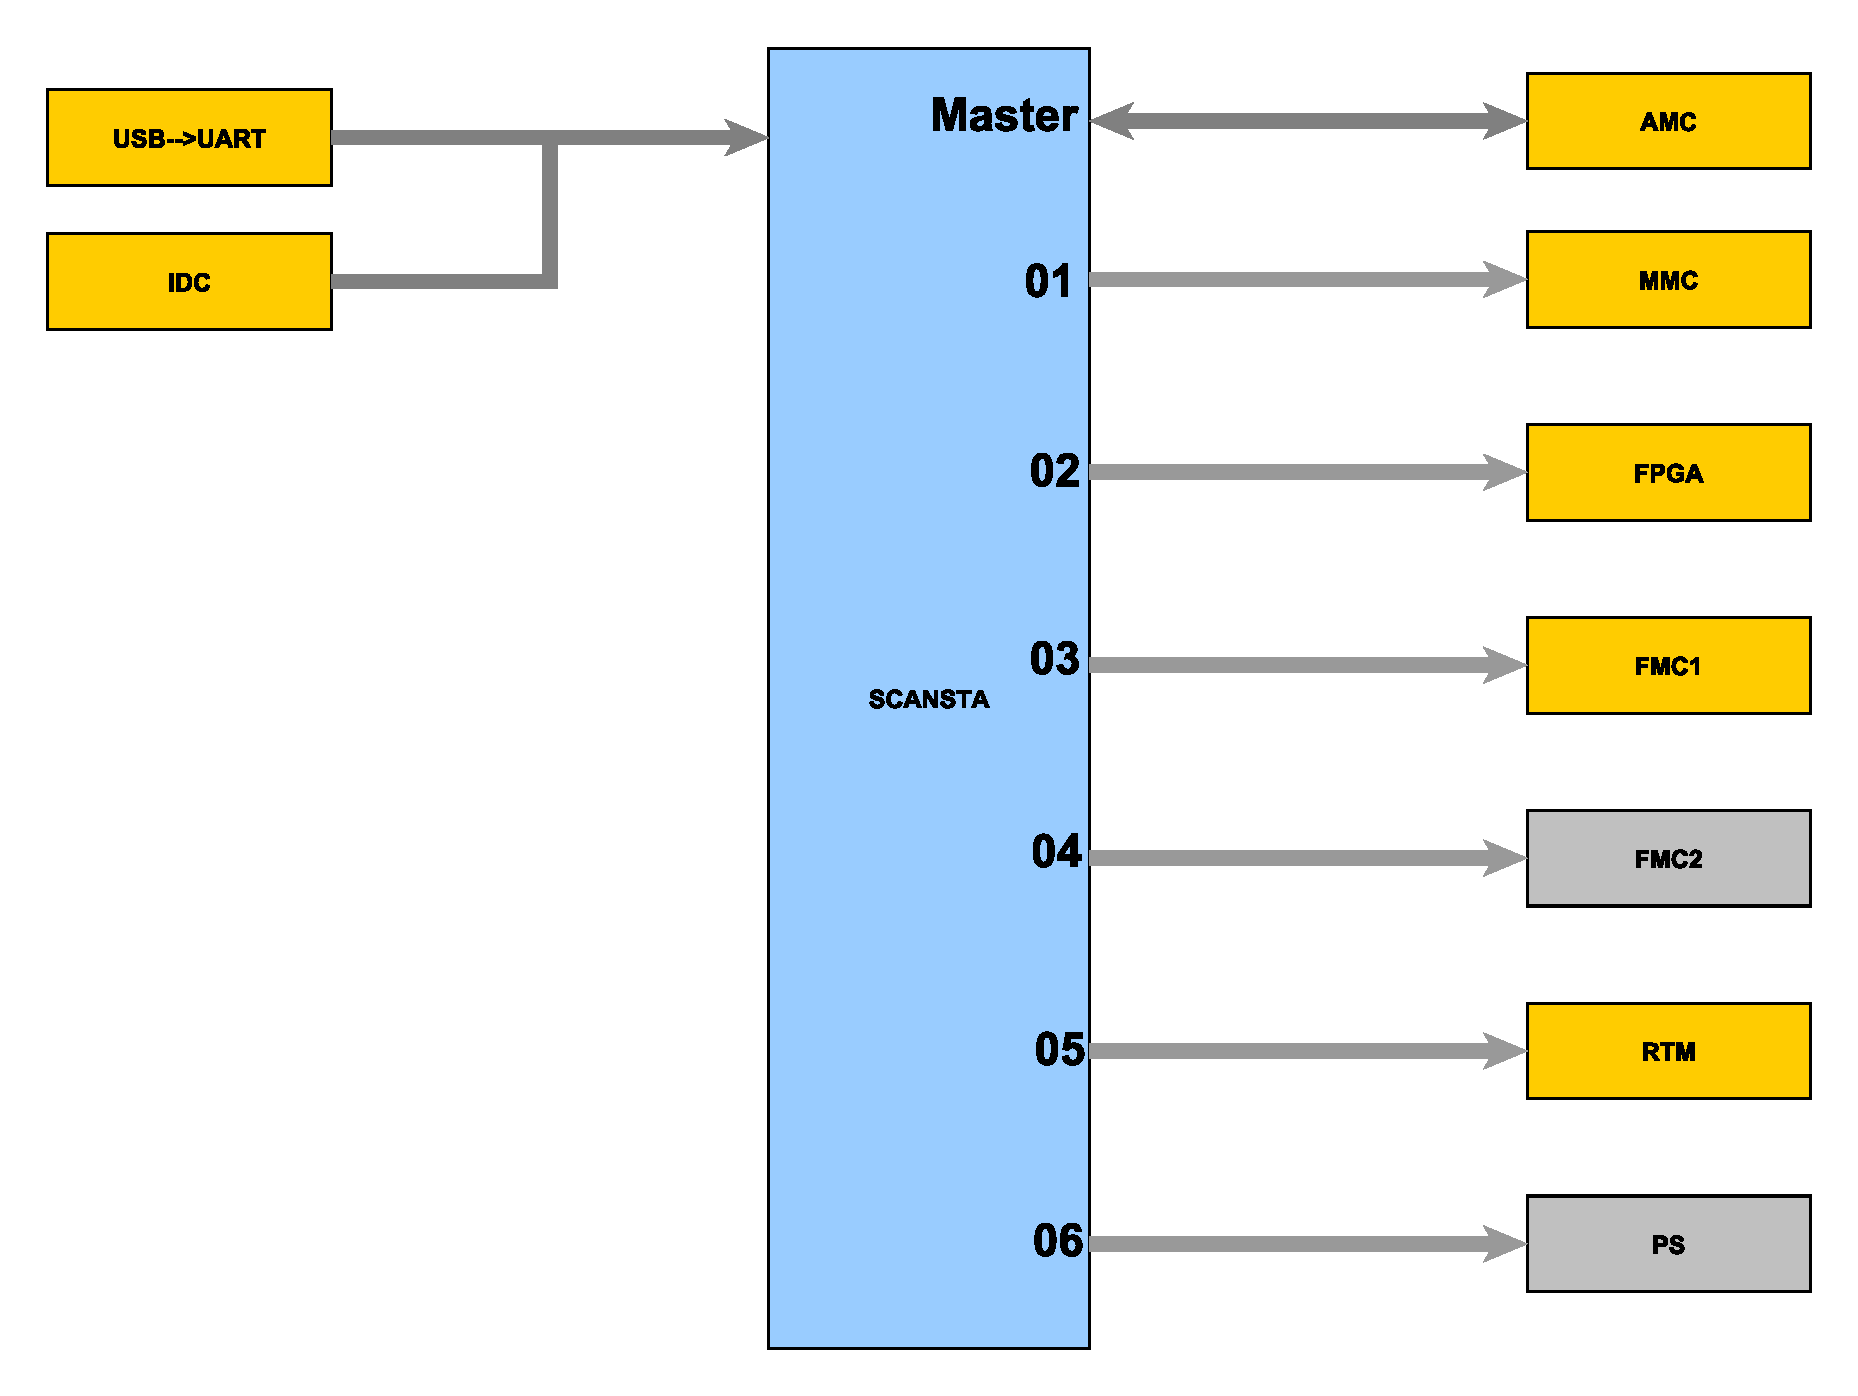
\includegraphics[scale=0.4]{img/scansta.eps}\\
			\caption{SCANSTA bloch scheme} 
		\end{figure}
		
	\textit{\textbf{Note:} The FMC2 and PS is not used.}\\


Each of JTAG slave devices is connected directly to SCANSTA. SCANSTA allows to connect all devices in chain witn an option to pass one or more devices, intention in Figure \ref{jtagchain}.

		\begin{figure}[htbp!]
			\centering
			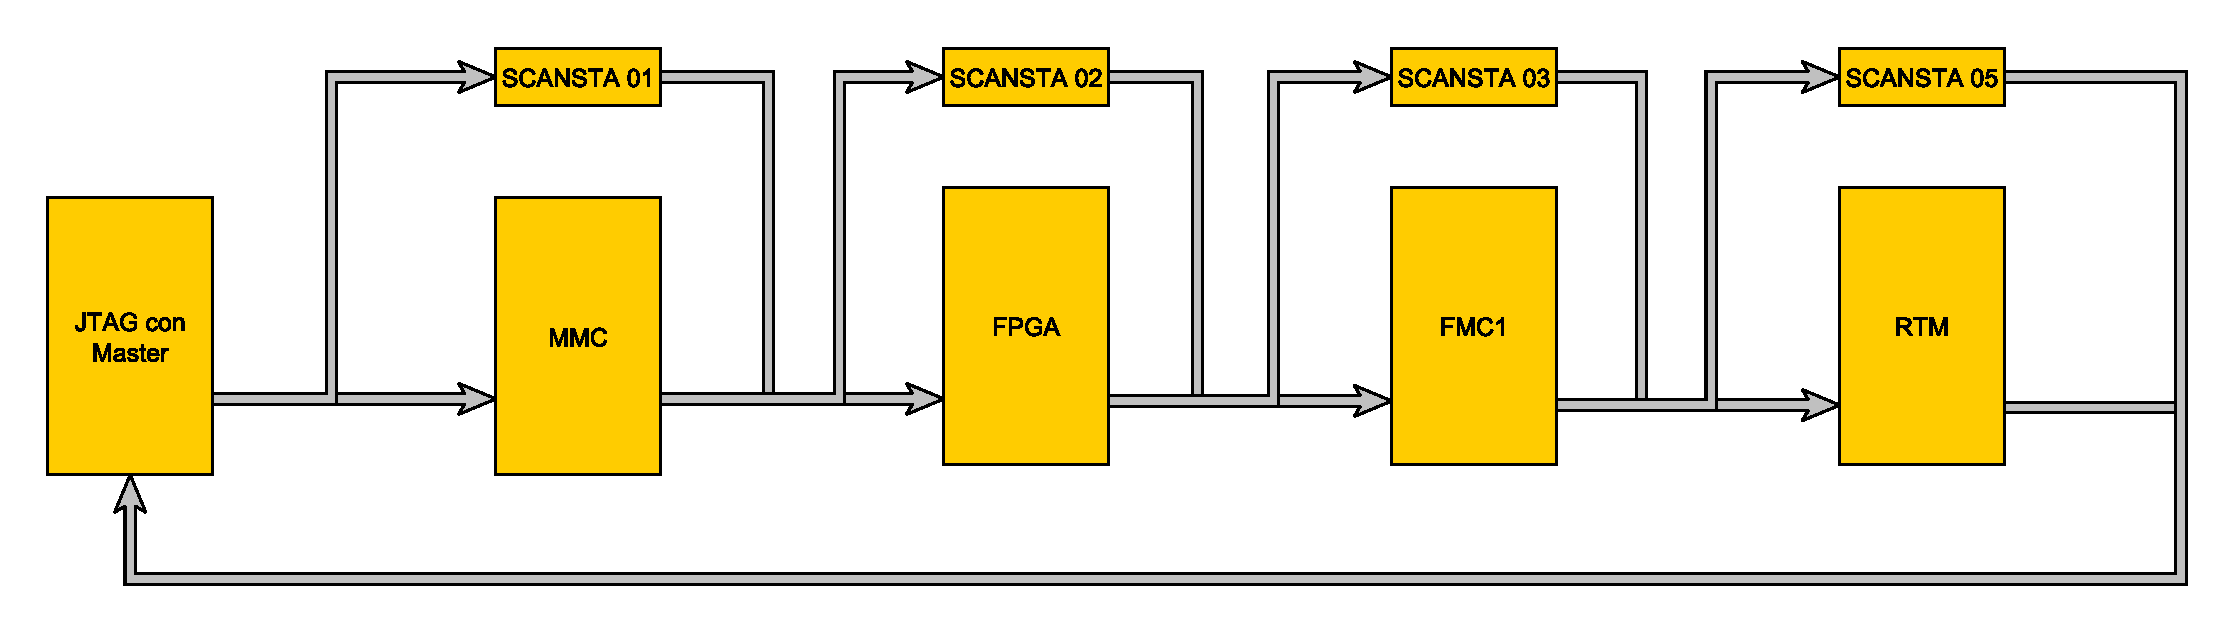
\includegraphics[scale=0.4]{img/jtagchain.eps}\\
			\caption{SCANSTA JTAG chain} \label{jtagchain}
		\end{figure}
		
		
Simplified instruction if using SCANSTA can be found under: \href{http://www.ti.com/lit/an/snla068c/snla068c.pdf}{http://www.ti.com/lit/an/snla068c/snla068c.pdf} 

\clearpage

\section{FPGA bootstrapping}


\noindent
\textbf{Xilinx User Guide:} \href{https://www.xilinx.com/support/documentation/user_guides/ug570-ultrascale-configuration.pdf}{https://www.xilinx.com/support/documentation/user\_guides/ug570-ultrascale-configuration.pdf}\\

To load FPGA .bit into flash Vivado in version minimum 16.4 is needed.\\
\textbf{Vivado WebPack:}\href{https://www.xilinx.com/support/download.html}{https://www.xilinx.com/support/download.html}

Alternatively Vivado Lab tools (previously Lab Tools) can be used.\\
\textbf{Vivado Lab Edition:}\href{https://www.xilinx.com/support/download.html}{https://www.xilinx.com/support/download.html}


\clearpage

\section{Power}
\subsection{Power supply}
The card can operate connested to SAYMA AMC card. When the card is inserted to the SAYMA AMC,  the power is applied from RTM connector -J2, +12V (4 power lines) and +3.3\_MP(1 line). Both voltages can be controlled by SAYMA AMC.
+12 is converted to lower voltages and negative voltages, simplified power map is in figure \ref{powermap}. There are few types of power distributors, fixed LDOs, Buck converters and Exar chip - quad channel digital Pulse Width Modulated (PWM) step down (buck) controller. Exar allows for adjust power parameters and for set particular power oorder. Exar firmware monitors current and responds if its too high.  Additionaly all LDOs have connected PowerGood outputs so it is possible to read the proper state of all power busses. 

\todo[inline]{TBD voltage noise}



%Maximum board(AMC+RTM module) power consumption estimate to 3A @ 12V.\\
%
%	\textit{\textbf{Note:} Please note that power consumption mostly depends from FPGA configuration. \\}

\begin{itemize}
 

\item Input voltage range: 10.8-13.2 [V]\\
\item The board needs active cooling. Approx. 20CFM in 20 C air.\\

\end{itemize}

Exar chips are configured via EXAR\_I2C bus (I2CMUX7) or directly by connecting to W1 
%(call-out 28) 
header. For proper configuration \textbf{Exar Power Architect} in version \textbf{5.2-r1} is needed.
% Configuration files can be found at github in folder \href{https://github.com/m-labs/sinara/tree/master/EXAR\_config}{m-labs/sinara/Exar\_config}\\

\noindent
\textbf{Exar Power Archtect 5.2-r1:}
\href{https://www.exar.com/content/document.ashx?id=21632}{https://www.exar.com/content/document.ashx?id=21632}\\
\textbf{Configuration files:}
\href{https://github.com/m-labs/sinara/tree/master/EXAR\_config}{https://github.com/m-labs/sinara/tree/master/EXAR\_config}\\
\textbf{Datasheet:}\href{https://www.exar.com/ds/xr77129_1a_120514.pdf}{https://www.exar.com/ds/xr77129\_1a\_120514.pdf}\\
\textbf{Quick Start Guide:} \href{https://www.exar.com/files/powerxr/PA5-QSG_110_010614.pdf}{https://www.exar.com/files/powerxr/PA5-QSG\_110\_010614.pdf}\\


Actual voltages and current consumption, temperature can be found in Chip Dashboard. There is also oportunity to adjust settings.

\begin{figure}[htbp!]
	\centering
	\includegraphics[scale=0.6]{img/exarprog.png}\\
	\caption{Chip Dashboard} 
\end{figure}

\clearpage
\subsection{Power configuration} 

\subsubsection{Power map}


	\begin{figure}[htbp!]
		\centering
		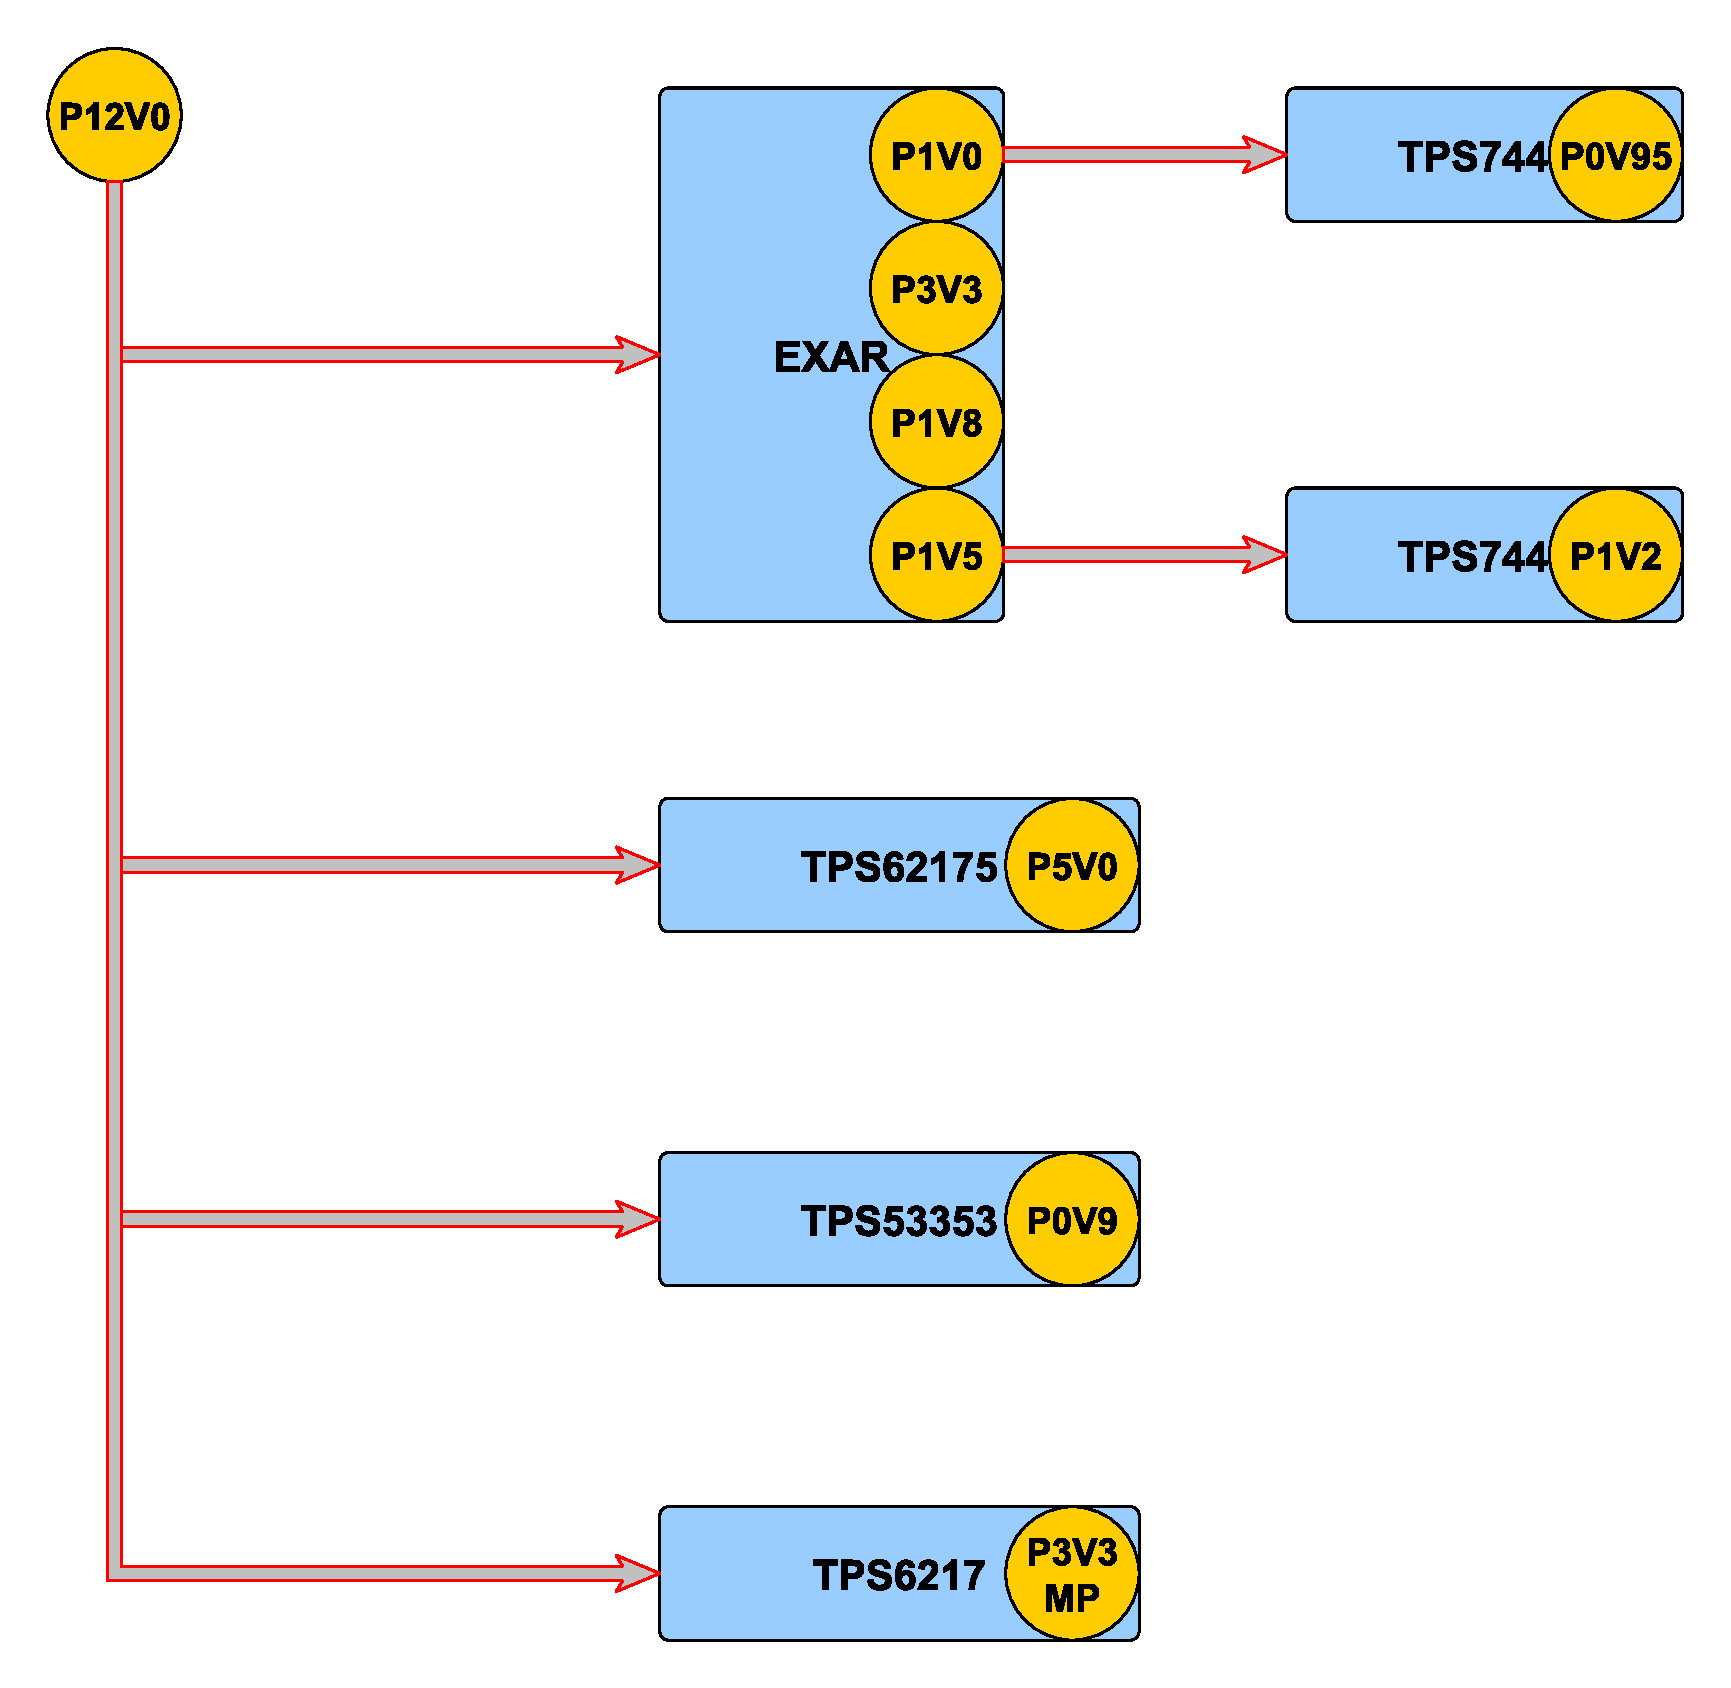
\includegraphics[scale=0.3]{img/pwr.eps}\\
		\caption{Power map} \label{powermap}
	\end{figure}
	

\begin{longtable}{|c|c|c|} \hline
\multicolumn{3}{|c|}{voltages and currents}	\\ \hline
P1V0 & 1.0V & 4A \\ \hline
P1V2 & 1.2V & 2A\\ \hline
P1V8 & 1.8V & 2A\\ \hline
P2V0 & 2.0V & 4A\\ \hline
P3V3 & 3.3V & 4A\\ \hline
P4V0 & 4.0V & 4A\\ \hline
P6V0 & 6.0V & 8A\\ \hline
P12V0A & 12.0V & 1A \\ \hline
N6V0A & -6.0V & 4A\\ \hline
N12V0A & -12.0V & 1A \\ \hline

\end{longtable}
	
\subsubsection{Exar parameters}

Exar chip(XR77129) has 4 configurable outputs with configirable current limits. Each channel can be confugured individually. It is possible to set voltage, current limit and power sequencing. In Figure \ref{exar1} we can see that main power supply is 12V, Under Voltage Lockout(UVLO) is set to 6V, so below this value chip will shutdown all channels. When the temperature rise under Over Temperature Protection (OTP) 105 degrees, the chip will generate warning event and restart. \\
All 4 channells can be grouped together and will start-up and shut-down in an user defined sequwnce. Selecting none means channels will not be assigned to any group and therefore, will be controlled independently. Group 0 is controlled by ENABLE or EXAR\_I2C command. Group 1 can be controlled by GPIO or by EXAR\_I2C command. By selecting 'Wait PGOOD' next channel will not power up untill current channel reaches the target level. Delay is an additional delay time which postpone after power up one and another channel in group.\\
In on-going Exar configuration - Figure \ref{exar2}, power sequencing looks like this: After Enable - EN\_DC\_DC, P1V0 start-up, after it reaches proper value, Exar turn ramp up another channel in this group - P3V3. In the same order are ramp up next two channels in this group.



	\begin{figure}[htbp!]
		\centering
		\includegraphics[scale=0.5]{img/exar1.png}\\
		\caption{Exar configuration} \label{exar1}
	\end{figure}
\clearpage	
	\begin{figure}[htbp!]
		\centering
		\includegraphics[scale=0.5]{img/exar2.png}\\
		\caption{Exar power on delays} \label{exar2}
	\end{figure}	
	



%\subsubsection{Exar configuration}
%Exar chips are configured via I2C bus (MUX Port 5) or directly by connecting to W1 (call-out 28) header. For proper configuration \textbf{Exar Power Architect} in version \textbf{5.2-r1} is needed.
%% Configuration files can be found at github in folder \href{https://github.com/m-labs/sinara/tree/master/EXAR\_config}{m-labs/sinara/Exar\_config}\\
%
%\noindent
%\textbf{Exar Power Archtect 5.2-r1:}
%\href{https://www.exar.com/content/document.ashx?id=21632}{https://www.exar.com/content/document.ashx?id=21632}\\
%\textbf{Configuration files:}
%\href{https://github.com/m-labs/sinara/tree/master/EXAR\_config}{https://github.com/m-labs/sinara/tree/master/EXAR\_config}\\
%\textbf{Datasheet:}\href{https://www.exar.com/ds/xr77129_1a_120514.pdf}{https://www.exar.com/ds/xr77129\_1a\_120514.pdf}\\
%\textbf{Quick Start Guide:} \href{https://www.exar.com/files/powerxr/PA5-QSG_110_010614.pdf}{https://www.exar.com/files/powerxr/PA5-QSG\_110\_010614.pdf}\\
%
%
%Actual voltages and current consumption, temperature can be found in Chip Dashboard. There is also oportunity to adjust settings.
%
%	\begin{figure}[htbp!]
%		\centering
%		\includegraphics[scale=0.6]{img/exarprog.png}\\
%		\caption{Chip Dashboard} 
%	\end{figure}
%
\subsection{Maximum power draw for each Mezzaninne}

\begin{longtable}{|c|c|} \hline
	Power rail[V] & Current [mA]\\ \hline
	+12 & 200 \\ \hline
	-12 & 50 \\ \hline
	+6 & 1500 \\ \hline
	-6 & 100 \\ \hline
	+3.3 & 1000 \\ \hline
	
\end{longtable}	

\clearpage

\section{MMC}

\subsection{MMC steps during booting}

\begin{itemize}

\item configures CPU, UART from own FLASH 
\item sets IO port directions
\item enables VCCINT PSU
\item enables P5V0 PSU (helper PSU)
\item enables Exar PSU. It boots from its own EEPROM
\item waits 200ms
\item configures SCANSTA chip in stitcher mode. If RTM is inserted, it enables its JTAG port
\item configures I2C switch base address for master ports - MMC, FPGA
\item initializes default RTM power state to off
\item initializes Ethernet PHY chip in RGMII mode using pin strap.
\item waits 200ms
\item initializes I2C controller and chain (switch)
\item configures Si5324
\item checks if RTM is inserted, if yes, then enables its power, waits 200ms and initializes RTM power supply via RTM\_I2C. It also configures Si5324 on RTM
\item runs task.\\
 
The task performs following functions:

\item checks if FPGA is configured. If not, it keeps Ethernet PHY in reset state. Once FPGA gets configured, it initializes the PHY.
\item checks if RTM is unplugged. If not, it switches the power off to make sure it is off during hotplug.
\end{itemize}
\textit{\textbf{Note:}Configuration CPU, UART does not affect with any changes of LED indicators.}


\subsection{Bootstraping}
To compile binaries \href{https://www.nxp.com/products/processors-and-microcontrollers/arm-based-processors-and-mcus/lpc-cortex-m-mcus/lpc1100-cortex-m0-plus-m0/lpcxpresso-ide-v8.2.2:LPCXPRESSO?tab=Design_Tools_Tab}{LPCXpresso} in newest version is needed.\\
\href{https://www.nxp.com/docs/en/user-guide/LPCXpresso_IDE_User_Guide.pdf}{LPCXpresso User Guide}

Another option is to compile under Linux using cmake toolchain in version 4.9.3.
\begin{lstlisting}
cmake & arm-none-eabi-gcc
\end{lstlisting}

\begin{itemize}
	\item Header flashing

The MMC can be upgraded by USB cable and NXP programmer(can be used other programmer but make sure that header shorts pins 3, 5, 9) using  \href{http://www.flashmagictool.com/}{Flashmagic} or any other software which can talk with NXP bootloader. The tested programmer is LPCLink V2. Flashing using programmer allows to debug.

	\item USB flashing
The MMC can be upgraded using USB and flashmagic software. This option only allows to flash IC, without any debug option.
Steps to flash using USB:
\begin{itemize}
	\item Set serial console 115200 8n1
	\item Press front-panel button -PB3 to trigger MMD to dump to serial console
	\item Set LPC1776, 8MHz oscillator, select hex file and press start
\end{itemize}

\end{itemize}

The source code is written in C and can be found on github.\\ 
\textbf{Source code:} \href{https://github.com/m-labs/sinara/tree/master/SAYMA\_firmware}{https://github.com/m-labs/sinara/tree/master/SAYMA\_firmware}.\\
\textbf{pre-compiled binary:} \href{https://github.com/m-labs/mmc-firmware/releases}{https://github.com/m-labs/mmc-firmware/releases}\\



%\subsection{Functionality}
%
%\todo[inline]{needed?}

\subsection{Exar debugging}
 
In case of chip failure, i.g.overvoltage, overcurrent, etc., there is possibility  to check chip status via UART. In this case in UART console, Exar register readout can be done by typing 'P' character.\\

	\begin{figure}[htbp!]
		\centering
		\includegraphics[scale=0.6]{img/exarreg.png}\\
		\caption{Exar register } 
	\end{figure}	
\clearpage
\subsection{PHY debugging}

In case of chip failure, there is possibility to check chip status via UART. In this case in UART console, Ethernet PHY content can be read by typing 'E' character

	\begin{figure}[htbp!]
		\centering
		\includegraphics[scale=0.6]{img/phyreg.png}\\
		\caption{Ethernet PHY register } 
	\end{figure}

\subsection{Ethernet }

There is no Ethernet sharing between MMC and FPGA due to speed difference between RGMII and RMII. PHY does not provide link speed translation.

\subsection{OpenMMC}

\textbf{OpenMMC Project:}\href{https://github.com/lnls-dig/openMMC}{https://github.com/lnls-dig/openMMC}

\todo[inline]{TBD}

\clearpage

\section{Housekeeping Signals}

\subsection{sensors}
Temperature:\\

\begin{longtable}{|c|c|c|c|c|}\hline
	\multicolumn{5}{|c|}{IPMI\_I2C}\\ \hline
	No & Addr. & placement & Type & Accuracy \\ \hline
	IC39 & 0x4A & Bottom - close to ADC  & LM75 & +/- 2 \\ \hline
	IC40 & 0x49 & Bottom - close to HMC7043 buffer& LM75 & +/- 2  \\ \hline
	IC44 & 0x24 & Bottom - under Mezzanine1 & MAX664A & +/- 1 \\ \hline
\end{longtable}

\begin{longtable}{|c|c|c|c|c|}\hline
		\multicolumn{5}{|c|}{TEMP\_SENS\_I2C}\\ \hline
	No & Addr. & placement & Type & Accuracy \\ \hline
	IC56 & 0x48 & Bottom - under DAC & ADT7420 & +/- 0.25 \\ \hline
	IC57 & 0x49 & Bottom center & ADT7420 & +/- 0.25  \\ \hline
\end{longtable}

All sensors are available either from AMC siede I2C or from RTM\_FPGA.
%All temperature sensors are tied tohether to one I2C bus - I2C\_SENS. \\







\subsection{Safety interlocks}

Temperature interlock is available on RTM board only and gets activated after reaching 80 degrees. This is hardware interlock and cannot be deactivated. Dedicated LED (LD15) gets on and RTM power supply is off until the temperature is exceeded
\clearpage


\section{Signal tables}
%---------------------------------------------------------SFP1
\begin{footnotesize}
	\begin{longtable}{|l|p{6cm}|p{6cm}|}
	\hline
	\multicolumn{3}{|c|}{\multirow{2}{*}{\textbf{\large{RTM}}}}\\
	\multicolumn{3}{|c|}{} \\ \hline 
	E3	&	MGTPRXN0\_216	&	RTM\_FPGA\_GTP\_Rx0\_N	\\ \hline
	E4	&	MGTPRXP0\_216	&	RTM\_FPGA\_GTP\_Rx0\_P	\\ \hline
	H1	&	MGTPTXN0\_216	&	RTM\_FPGA\_GTP\_Tx0C\_N	\\ \hline
	H2	&	MGTPTXP0\_216	&	RTM\_FPGA\_GTP\_Tx0C\_P	\\ \hline
	A3	&	MGTPRXN1\_216	&	RTM\_FPGA\_GTP\_Rx1\_N	\\ \hline
	A4	&	MGTPRXP1\_216	&	RTM\_FPGA\_GTP\_Rx1\_P	\\ \hline
	F1	&	MGTPTXN1\_216	&	RTM\_FPGA\_GTP\_Tx1C\_N	\\ \hline
	F2	&	MGTPTXP1\_216	&	RTM\_FPGA\_GTP\_Tx1C\_P	\\ \hline
	C3	&	MGTPRXN2\_216	&	RTM\_FPGA\_GTP\_Rx2\_N	\\ \hline
	C4	&	MGTPRXP2\_216	&	RTM\_FPGA\_GTP\_Rx2\_P	\\ \hline
	D1	&	MGTPTXN2\_216	&	RTM\_FPGA\_GTP\_Tx2C\_N	\\ \hline
	D2	&	MGTPTXP2\_216	&	RTM\_FPGA\_GTP\_Tx2C\_P	\\ \hline
	G3	&	MGTPRXN3\_216	&	RTM\_FPGA\_GTP\_Rx3\_N	\\ \hline
	G4	&	MGTPRXP3\_216	&	RTM\_FPGA\_GTP\_Rx3\_P	\\ \hline
	B1	&	MGTPTXN3\_216	&	RTM\_FPGA\_GTP\_Tx3C\_N	\\ \hline
	B2	&	MGTPTXP3\_216	&	RTM\_FPGA\_GTP\_Tx3C\_P	\\ \hline
	D5	&	MGTREFCLK0N\_216	&	RTM\_FPGA\_GTP\_CLKC\_P	\\ \hline
	D6	&	MGTREFCLK0P\_216	&	RTM\_FPGA\_GTP\_CLKC\_N	\\ \hline
	J6	&	IO\_0\_34	&	RTM\_FPGA\_SCL	\\ \hline
	K6	&	IO\_L1P\_T0\_34	&	RTM\_FPGA\_SDA	\\ \hline
	P14	&	IO\_L12P\_T1\_MRCC\_14	&	RTM\_MASTER\_AUX\_CLK\_P	\\ \hline
	R15	&	IO\_L12N\_T1\_MRCC\_14	&	RTM\_MASTER\_AUX\_CLK\_N	\\ \hline
	R16	&	IO\_L14P\_T2\_SRCC\_14	&	RTM\_FPGA\_LVDS1\_P	\\ \hline
	R17	&	IO\_L14N\_T2\_SRCC\_14	&	RTM\_FPGA\_LVDS1\_N	\\ \hline
	T17	&	IO\_L16P\_T2\_CSI\_B\_14	&	RTM\_FPGA\_LVDS2\_P	\\ \hline
	U17	&	IO\_L16N\_T2\_A15\_D31\_14	&	RTM\_FPGA\_LVDS2\_N	\\ \hline
	T18	&	IO\_L15N\_T2\_DQS\_DOUT\_CSO\_B\_14	&	RTM\_FPGA\_USR\_IO\_N	\\ \hline
	P14	&	IO\_L12P\_T1\_MRCC\_14	&	RTM\_MASTER\_AUX\_CLK\_P	\\ \hline
	R15	&	IO\_L12N\_T1\_MRCC\_14	&	RTM\_MASTER\_AUX\_CLK\_N	\\ \hline
	
		
	\end{longtable}
\end{footnotesize}

%---------------------------------------------------------Mez1
\begin{footnotesize}
	\begin{longtable}{|l|p{6cm}|p{6cm}|}
		\hline
		\multicolumn{3}{|c|}{\multirow{2}{*}{\textbf{\large{Mezzanine1 IO}}}}\\
		\multicolumn{3}{|c|}{} \\ \hline 
P1	&	IO\_L9N\_T1\_DQS\_34	&	MEZZ1\_IO0	\\ \hline
M4	&	IO\_L10P\_T1\_34	&	MEZZ1\_IO1	\\ \hline
N4	&	IO\_L10N\_T1\_34	&	MEZZ1\_IO2	\\ \hline
N3	&	IO\_L11P\_T1\_SRCC\_34	&	MEZZ1\_IO3	\\ \hline
N2	&	IO\_L11N\_T1\_SRCC\_34	&	MEZZ1\_IO4	\\ \hline
P4	&	IO\_L12P\_T1\_MRCC\_34	&	MEZZ1\_IO5	\\ \hline
P3	&	IO\_L12N\_T1\_MRCC\_34	&	MEZZ1\_IO6	\\ \hline
R2	&	IO\_L13P\_T2\_MRCC\_34	&	MEZZ1\_IO7	\\ \hline
R1	&	IO\_L13N\_T2\_MRCC\_34	&	MEZZ1\_IO8	\\ \hline
R3	&	IO\_L14P\_T2\_SRCC\_34	&	MEZZ1\_IO9	\\ \hline
T2	&	IO\_L14N\_T2\_SRCC\_34	&	MEZZ1\_IO10	\\ \hline
U2	&	IO\_L15P\_T2\_DQS\_34	&	MEZZ1\_IO11	\\ \hline
U1	&	IO\_L15N\_T2\_DQS\_34	&	MEZZ1\_IO12	\\ \hline
V3	&	IO\_L16P\_T2\_34	&	MEZZ1\_IO13	\\ \hline
V2	&	IO\_L16N\_T2\_34	&	MEZZ1\_IO14	\\ \hline
T4	&	IO\_L17P\_T2\_34	&	MEZZ1\_IO15	\\ \hline
	
	\end{longtable}
\end{footnotesize}

%---------------------------------------------------------mezz2
\begin{footnotesize}
	\begin{longtable}{|l|p{6cm}|p{6cm}|}
		\hline
		\multicolumn{3}{|c|}{\multirow{2}{*}{\textbf{\large{Mezzanine2 IO}}}}\\
		\multicolumn{3}{|c|}{} \\ \hline 
T3	&	IO\_L17N\_T2\_34	&	MEZZ2\_IO0	\\ \hline
U4	&	IO\_L18P\_T2\_34	&	MEZZ2\_IO1	\\ \hline
V4	&	IO\_L18N\_T2\_34	&	MEZZ2\_IO2	\\ \hline
P6	&	IO\_L19P\_T3\_34	&	MEZZ2\_IO3	\\ \hline
P5	&	IO\_L19N\_T3\_VREF\_34	&	MEZZ2\_IO4	\\ \hline
U6	&	IO\_L20P\_T3\_34	&	MEZZ2\_IO5	\\ \hline
U5	&	IO\_L20N\_T3\_34	&	MEZZ2\_IO6	\\ \hline
R5	&	IO\_L21P\_T3\_DQS\_34	&	MEZZ2\_IO7	\\ \hline
T5	&	IO\_L21N\_T3\_DQS\_34	&	MEZZ2\_IO8	\\ \hline
R7	&	IO\_L22P\_T3\_34	&	MEZZ2\_IO9	\\ \hline
T7	&	IO\_L22N\_T3\_34	&	MEZZ2\_IO10	\\ \hline
U7	&	IO\_L23P\_T3\_34	&	MEZZ2\_IO11	\\ \hline
V6	&	IO\_L23N\_T3\_34	&	MEZZ2\_IO12	\\ \hline
V8	&	IO\_L24P\_T3\_34	&	MEZZ2\_IO13	\\ \hline
V7	&	IO\_L24N\_T3\_34	&	MEZZ2\_IO14	\\ \hline
R6	&	IO\_25\_34	&	MEZZ2\_IO15	\\ \hline
	
	\end{longtable}
\end{footnotesize}

%---------------------------------------------------------mezz3
\begin{footnotesize}
	\begin{longtable}{|l|p{6cm}|p{6cm}|}
		\hline
		\multicolumn{3}{|c|}{\multirow{2}{*}{\textbf{\large{Mezzanine3 IO}}}}\\
		\multicolumn{3}{|c|}{} \\ \hline 
D11	&	IO\_L6P\_T0\_15	&	MEZZ3\_IO0	\\ \hline
C12	&	IO\_L6N\_T0\_VREF\_15	&	MEZZ3\_IO1	\\ \hline
B12	&	IO\_L7P\_T1\_AD2P\_15	&	MEZZ3\_IO2	\\ \hline
A12	&	IO\_L7N\_T1\_AD2N\_15	&	MEZZ3\_IO3	\\ \hline
A13	&	IO\_L8P\_T1\_AD10P\_15	&	MEZZ3\_IO4	\\ \hline
A14	&	IO\_L8N\_T1\_AD10N\_15	&	MEZZ3\_IO5	\\ \hline
C14	&	IO\_L9P\_T1\_DQS\_AD3P\_15	&	MEZZ3\_IO6	\\ \hline
B15	&	IO\_L9N\_T1\_DQS\_AD3N\_15	&	MEZZ3\_IO7	\\ \hline
B14	&	IO\_L10P\_T1\_AD11P\_15	&	MEZZ3\_IO8	\\ \hline
A15	&	IO\_L10N\_T1\_AD11N\_15	&	MEZZ3\_IO9	\\ \hline
D13	&	IO\_L11P\_T1\_SRCC\_15	&	MEZZ3\_IO10	\\ \hline
C13	&	IO\_L11N\_T1\_SRCC\_15	&	MEZZ3\_IO11	\\ \hline
E13	&	IO\_L12P\_T1\_MRCC\_15	&	MEZZ3\_IO12	\\ \hline
D14	&	IO\_L12N\_T1\_MRCC\_15	&	MEZZ3\_IO13	\\ \hline
D15	&	IO\_L13N\_T2\_MRCC\_15	&	MEZZ3\_IO14	\\ \hline
E16	&	IO\_L14P\_T2\_SRCC\_15	&	MEZZ3\_IO15	\\ \hline

	\end{longtable}
\end{footnotesize}


%---------------------------------------------------------mezz4
\begin{footnotesize}
	\begin{longtable}{|l|p{6cm}|p{6cm}|}
		\hline
		\multicolumn{3}{|c|}{\multirow{2}{*}{\textbf{\large{Mezzanine4 IO}}}}\\
		\multicolumn{3}{|c|}{} \\ \hline 
K5	&	IO\_L1N\_T0\_34	&	MEZZ4\_IO0	\\ \hline
J5	&	IO\_L2P\_T0\_34	&	MEZZ4\_IO1	\\ \hline
J4	&	IO\_L2N\_T0\_34	&	MEZZ4\_IO2	\\ \hline
K2	&	IO\_L3P\_T0\_DQS\_34	&	MEZZ4\_IO3	\\ \hline
K1	&	IO\_L3N\_T0\_DQS\_34	&	MEZZ4\_IO4	\\ \hline
K3	&	IO\_L4P\_T0\_34	&	MEZZ4\_IO5	\\ \hline
L2	&	IO\_L4N\_T0\_34	&	MEZZ4\_IO6	\\ \hline
L4	&	IO\_L5P\_T0\_34	&	MEZZ4\_IO7	\\ \hline
L3	&	IO\_L5N\_T0\_34	&	MEZZ4\_IO8	\\ \hline
L5	&	IO\_L6P\_T0\_34	&	MEZZ4\_IO9	\\ \hline
M5	&	IO\_L6N\_T0\_VREF\_34	&	MEZZ4\_IO10	\\ \hline
M2	&	IO\_L7P\_T1\_34	&	MEZZ4\_IO11	\\ \hline
M1	&	IO\_L7N\_T1\_34	&	MEZZ4\_IO12	\\ \hline
M6	&	IO\_L8P\_T1\_34	&	MEZZ4\_IO13	\\ \hline
N6	&	IO\_L8N\_T1\_34	&	MEZZ4\_IO14	\\ \hline
N1	&	IO\_L9P\_T1\_DQS\_34	&	MEZZ4\_IO15	\\ \hline

		
	\end{longtable}
\end{footnotesize}


%---------------------------------------------------------clk
\begin{footnotesize}
	\begin{longtable}{|l|p{6cm}|p{6cm}|}
		\hline
		\multicolumn{3}{|c|}{\multirow{2}{*}{\textbf{\large{Mezzanine CLK IO}}}}\\
		\multicolumn{3}{|c|}{} \\ \hline 
D18	&	IO\_L17N\_T2\_A25\_15	&	CLK\_MEZZ\_IO0	\\ \hline
C17	&	IO\_L18P\_T2\_A24\_15	&	CLK\_MEZZ\_IO1	\\ \hline
C18	&	IO\_L18N\_T2\_A23\_15	&	CLK\_MEZZ\_IO2	\\ \hline
G17	&	IO\_L19P\_T3\_A22\_15	&	CLK\_MEZZ\_IO3	\\ \hline
F18	&	IO\_L19N\_T3\_A21\_VREF\_15	&	CLK\_MEZZ\_IO4	\\ \hline
H16	&	IO\_L20P\_T3\_A20\_15	&	CLK\_MEZZ\_IO5	\\ \hline
G16	&	IO\_L20N\_T3\_A19\_15	&	CLK\_MEZZ\_IO6	\\ \hline
G15	&	IO\_L21P\_T3\_DQS\_15	&	CLK\_MEZZ\_IO7	\\ \hline
F15	&	IO\_L21N\_T3\_DQS\_A18\_15	&	CLK\_MEZZ\_IO8	\\ \hline
G14	&	IO\_L22P\_T3\_A17\_15	&	CLK\_MEZZ\_IO9	\\ \hline
F14	&	IO\_L22N\_T3\_A16\_15	&	CLK\_MEZZ\_IO10	\\ \hline
H17	&	IO\_L23P\_T3\_FOE\_B\_15	&	CLK\_MEZZ\_IO11	\\ \hline
H18	&	IO\_L23N\_T3\_FWE\_B\_15	&	CLK\_MEZZ\_IO12	\\ \hline
F17	&	IO\_L24P\_T3\_RS1\_15	&	CLK\_MEZZ\_IO13	\\ \hline
H14	&	IO\_25\_15	&	CLK\_MEZZ\_IO14	\\ \hline
&	IO\_L24N\_T3\_RS0\_15	&	CLK\_MEZZ\_IO15	\\ \hline

		
		
	\end{longtable}
\end{footnotesize}
\clearpage

\section{Factory acceptance testing}

TBD
\clearpage


\begin{appendix}

\section{Total table of signals}

\begin{footnotesize}
	\begin{longtable}{|l|p{6cm}|p{6cm}|}
		\hline
%		\multicolumn{3}{|c|}{\multirow{2}{*}{\textbf{\large{Table 12 - FMC }}}} \\
FPGA ball	&	FPGA signal	&	Signal on the board	\\ \hline

A1	&	GND	&	GND	\\ \hline
A2	&	MGTAVTT	&	MGTAVTT	\\ \hline
A3	&	MGTPRXN1\_216	&	RTM\_FPGA\_GTP\_Rx1\_N	\\ \hline
A4	&	MGTPRXP1\_216	&	RTM\_FPGA\_GTP\_Rx1\_P	\\ \hline
A5	&	GND\_3	&	GND	\\ \hline
A6	&	MGTRREF\_216	&	NC	\\ \hline
A7	&	GND\_4	&	GND	\\ \hline
A8	&	GND\_5	&	GND	\\ \hline
A9	&	IO\_L3N\_T0\_DQS\_AD1N\_15	&	CAL\_ADC\_MCLK1	\\ \hline
A10	&	IO\_L5N\_T0\_AD9N\_15	&	CAL\_ADC\_CSn	\\ \hline
A11	&	GND\_1	&	GND	\\ \hline
A12	&	IO\_L7N\_T1\_AD2N\_15	&	MEZZ3\_IO3	\\ \hline
A13	&	IO\_L8P\_T1\_AD10P\_15	&	MEZZ3\_IO4	\\ \hline
A14	&	IO\_L8N\_T1\_AD10N\_15	&	MEZZ3\_IO5	\\ \hline
A15	&	IO\_L10N\_T1\_AD11N\_15	&	MEZZ3\_IO9	\\ \hline
A16	&	VCCO\_15	&	P3V3F	\\ \hline
A17	&	IO\_L15N\_T2\_DQS\_ADV\_B\_15	&	HMC\_SPI\_SCLK	\\ \hline
A18	&	GND\_2	&	GND	\\ \hline
B1	&	MGTPTXN3\_216	&	RTM\_FPGA\_GTP\_Tx3C\_N	\\ \hline
B2	&	MGTPTXP3\_216	&	RTM\_FPGA\_GTP\_Tx3C\_P	\\ \hline
B3	&	GND\_7	&	GND	\\ \hline
B4	&	MGTAVCC	&	MGTAVCC	\\ \hline
B5	&	MGTREFCLK1N\_216	&	CDR\_CLK\_CLEAN1\_N	\\ \hline
B6	&	MGTREFCLK1P\_216	&	CDR\_CLK\_CLEAN1\_P	\\ \hline
B7	&	GND\_8	&	GND	\\ \hline
B8	&	GND\_9	&	GND	\\ \hline
B9	&	IO\_L3P\_T0\_DQS\_AD1P\_15	&	CAL\_ADC\_MCLK2	\\ \hline
B10	&	IO\_L5P\_T0\_AD9P\_15	&	CAL\_ADC\_SYNCn	\\ \hline
B11	&	IO\_L4N\_T0\_15	&	CAL\_ADC\_DIN	\\ \hline
B12	&	IO\_L7P\_T1\_AD2P\_15	&	MEZZ3\_IO2	\\ \hline
B13	&	VCCO\_15\_1	&	P3V3F	\\ \hline
B14	&	IO\_L10P\_T1\_AD11P\_15	&	MEZZ3\_IO8	\\ \hline
B15	&	IO\_L9N\_T1\_DQS\_AD3N\_15	&	MEZZ3\_IO7	\\ \hline
B16	&	IO\_L15P\_T2\_DQS\_15	&	HMC\_SPI\_SDATA	\\ \hline
B17	&	IO\_L16N\_T2\_A27\_15	&	USR\_UART\_N	\\ \hline
B18	&	GND\_6	&	GND	\\ \hline
C1	&	MGTAVTT\_1	&	MGTAVTT	\\ \hline
C2	&	GND\_11	&	GND	\\ \hline
C3	&	MGTPRXN2\_216	&	RTM\_FPGA\_GTP\_Rx2\_N	\\ \hline
C4	&	MGTPRXP2\_216	&	RTM\_FPGA\_GTP\_Rx2\_P	\\ \hline
C5	&	MGTAVCC\_1	&	MGTAVCC	\\ \hline
C6	&	GND\_12	&	GND	\\ \hline
C7	&	GND\_13	&	GND	\\ \hline
C8	&	IO\_L1N\_T0\_AD0N\_15	&	HMC830\_SPI\_SEN	\\ \hline
C9	&	IO\_L2N\_T0\_AD8N\_15	&	CAL\_ADC\_SCLK	\\ \hline
C10	&	VCCO\_15\_2	&	P3V3F	\\ \hline
C11	&	IO\_L4P\_T0\_15	&	CAL\_ADC\_DOUT	\\ \hline
C12	&	IO\_L6N\_T0\_VREF\_15	&	MEZZ3\_IO1	\\ \hline
C13	&	IO\_L11N\_T1\_SRCC\_15	&	MEZZ3\_IO11	\\ \hline
C14	&	IO\_L9P\_T1\_DQS\_AD3P\_15	&	MEZZ3\_IO6	\\ \hline
C15	&	GND\_10	&	GND	\\ \hline
C16	&	IO\_L16P\_T2\_A28\_15	&	USR\_UART\_P	\\ \hline
C17	&	IO\_L18P\_T2\_A24\_15	&	CLK\_MEZZ\_IO1	\\ \hline
C18	&	IO\_L18N\_T2\_A23\_15	&	CLK\_MEZZ\_IO2	\\ \hline
D1	&	MGTPTXN2\_216	&	RTM\_FPGA\_GTP\_Tx2C\_N	\\ \hline
D2	&	MGTPTXP2\_216	&	RTM\_FPGA\_GTP\_Tx2C\_P	\\ \hline
D3	&	GND\_15	&	GND	\\ \hline
D4	&	GND\_16	&	GND	\\ \hline
D5	&	MGTREFCLK0N\_216	&	RTM\_FPGA\_GTP\_CLKC\_P	\\ \hline
D6	&	MGTREFCLK0P\_216	&	RTM\_FPGA\_GTP\_CLKC\_N	\\ \hline
D7	&	GND\_17	&	GND	\\ \hline
D8	&	IO\_L1P\_T0\_AD0P\_15	&	HMC\_SPI\_GPIO	\\ \hline
D9	&	IO\_L2P\_T0\_AD8P\_15	&	HMC\_SPI\_SDO	\\ \hline
D10	&	IO\_0\_15	&	SI5324\_INT\_ALM	\\ \hline
D11	&	IO\_L6P\_T0\_15	&	MEZZ3\_IO0	\\ \hline
D12	&	GND\_14	&	GND	\\ \hline
D13	&	IO\_L11P\_T1\_SRCC\_15	&	MEZZ3\_IO10	\\ \hline
D14	&	IO\_L12N\_T1\_MRCC\_15	&	MEZZ3\_IO13	\\ \hline
D15	&	IO\_L13N\_T2\_MRCC\_15	&	MEZZ3\_IO14	\\ \hline
D16	&	IO\_L14N\_T2\_SRCC\_15	&	HMC7043\_SLEN	\\ \hline
D17	&	VCCO\_15\_3	&	P3V3F	\\ \hline
D18	&	IO\_L17N\_T2\_A25\_15	&	CLK\_MEZZ\_IO0	\\ \hline
E1	&	MGTAVTT\_2	&	MGTAVTT	\\ \hline
E2	&	GND\_18	&	GND	\\ \hline
E3	&	MGTPRXN0\_216	&	RTM\_FPGA\_GTP\_Rx0\_N	\\ \hline
E4	&	MGTPRXP0\_216	&	RTM\_FPGA\_GTP\_Rx0\_P	\\ \hline
E5	&	MGTAVCC\_2	&	MGTAVCC	\\ \hline
E6	&	GND\_19	&	GND	\\ \hline
E7	&	GND\_20	&	GND	\\ \hline
E8	&	CCLK\_0	&	FPGA\_CFG\_CCLK	\\ \hline
E9	&	GND\_21	&	GND	\\ \hline
E10	&	VCCO\_0	&	P3V3F	\\ \hline
E11	&	VCCBATT\_0	&	P1V8F	\\ \hline
E12	&	CFGBVS\_0	&	NC	\\ \hline
E13	&	IO\_L12P\_T1\_MRCC\_15	&	MEZZ3\_IO12	\\ \hline
E14	&	VCCO\_15\_4	&	P3V3F	\\ \hline
E15	&	IO\_L13P\_T2\_MRCC\_15	&	NC	\\ \hline
E16	&	IO\_L14P\_T2\_SRCC\_15	&	MEZZ3\_IO15	\\ \hline
E17	&	IO\_L17P\_T2\_A26\_15	&	SI5324\_RST	\\ \hline
E18	&	IO\_L24N\_T3\_RS0\_15	&	CLK\_MEZZ\_IO15	\\ \hline
F1	&	MGTPTXN1\_216	&	RTM\_FPGA\_GTP\_Tx1C\_N	\\ \hline
F2	&	MGTPTXP1\_216	&	RTM\_FPGA\_GTP\_Tx1C\_P	\\ \hline
F3	&	MGTAVTT\_3	&	MGTAVTT	\\ \hline
F4	&	GND\_24	&	GND	\\ \hline
F5	&	MGTAVCC\_3	&	MGTAVCC	\\ \hline
F6	&	GND\_25	&	GND	\\ \hline
F7	&	VCCINT	&	P1V0	\\ \hline
F8	&	TCK\_0	&	TCK	\\ \hline
F9	&	VCCINT\_1	&	P1V0	\\ \hline
F10	&	GND\_22	&	GND	\\ \hline
F11	&	VCCBRAM	&	VCCBRAM	\\ \hline
F12	&	DONE\_0	&	FPGA\_CFG\_DONE	\\ \hline
F13	&	M2\_0	&	NC	\\ \hline
F14	&	IO\_L22N\_T3\_A16\_15	&	CLK\_MEZZ\_IO10	\\ \hline
F15	&	IO\_L21N\_T3\_DQS\_A18\_15	&	CLK\_MEZZ\_IO8	\\ \hline
F16	&	GND\_23	&	GND	\\ \hline
F17	&	IO\_L24P\_T3\_RS1\_15	&	CLK\_MEZZ\_IO13	\\ \hline
F18	&	IO\_L19N\_T3\_A21\_VREF\_15	&	CLK\_MEZZ\_IO4	\\ \hline
G1	&	GND\_26	&	GND	\\ \hline
G2	&	MGTAVTT\_4	&	MGTAVTT	\\ \hline
G3	&	MGTPRXN3\_216	&	RTM\_FPGA\_GTP\_Rx3\_N	\\ \hline
G4	&	MGTPRXP3\_216	&	RTM\_FPGA\_GTP\_Rx3\_P	\\ \hline
G5	&	GND\_29	&	GND	\\ \hline
G6	&	GND\_30	&	GND	\\ \hline
G7	&	GND\_31	&	GND	\\ \hline
G8	&	VCCINT\_2	&	P1V0	\\ \hline
G9	&	GND\_32	&	GND	\\ \hline
G10	&	VCCBRAM\_1	&	VCCBRAM	\\ \hline
G11	&	GND\_27	&	GND	\\ \hline
G12	&	VCCAUX	&	VCCAUX	\\ \hline
G13	&	GND\_28	&	GND	\\ \hline
G14	&	IO\_L22P\_T3\_A17\_15	&	CLK\_MEZZ\_IO9	\\ \hline
G15	&	IO\_L21P\_T3\_DQS\_15	&	CLK\_MEZZ\_IO7	\\ \hline
G16	&	IO\_L20N\_T3\_A19\_15	&	CLK\_MEZZ\_IO6	\\ \hline
G17	&	IO\_L19P\_T3\_A22\_15	&	CLK\_MEZZ\_IO3	\\ \hline
G18	&	VCCO\_15\_5	&	P3V3F	\\ \hline
H1	&	MGTPTXN0\_216	&	RTM\_FPGA\_GTP\_Tx0C\_N	\\ \hline
H2	&	MGTPTXP0\_216	&	RTM\_FPGA\_GTP\_Tx0C\_P	\\ \hline
H3	&	GND\_35	&	GND	\\ \hline
H4	&	GND\_36	&	GND	\\ \hline
H5	&	GND\_37	&	GND	\\ \hline
H6	&	GND\_38	&	GND	\\ \hline
H7	&	VCCINT\_3	&	P1V0	\\ \hline
H8	&	GND\_39	&	GND	\\ \hline
H9	&	VCCINT\_4	&	P1V0	\\ \hline
H10	&	GND\_33	&	GND	\\ \hline
H11	&	VCCBRAM\_2	&	VCCBRAM	\\ \hline
H12	&	GND\_34	&	GND	\\ \hline
H13	&	VCCAUX\_1	&	VCCAUX	\\ \hline
H14	&	IO\_25\_15	&	CLK\_MEZZ\_IO14	\\ \hline
H15	&	VCCO\_15\_6	&	P3V3F	\\ \hline
H16	&	IO\_L20P\_T3\_A20\_15	&	CLK\_MEZZ\_IO5	\\ \hline
H17	&	IO\_L23P\_T3\_FOE\_B\_15	&	CLK\_MEZZ\_IO11	\\ \hline
H18	&	IO\_L23N\_T3\_FWE\_B\_15	&	CLK\_MEZZ\_IO12	\\ \hline
J1	&	GND\_40	&	GND	\\ \hline
J2	&	GND\_44	&	GND	\\ \hline
J3	&	GND\_45	&	GND	\\ \hline
J4	&	IO\_L2N\_T0\_34	&	MEZZ4\_IO2	\\ \hline
J5	&	IO\_L2P\_T0\_34	&	MEZZ4\_IO1	\\ \hline
J6	&	IO\_0\_34	&	RTM\_FPGA\_SCL	\\ \hline
J7	&	GND\_46	&	GND	\\ \hline
J8	&	VCCINT\_6	&	P1V0	\\ \hline
J9	&	GNDADC\_0	&	NC	\\ \hline
J10	&	VCCADC\_0	&	NC	\\ \hline
J11	&	GND\_41	&	GND	\\ \hline
J12	&	VCCINT\_5	&	P1V0	\\ \hline
J13	&	GND\_42	&	GND	\\ \hline
J14	&	IO\_L5P\_T0\_D06\_14	&	REF\_CLK\_SRC\_SEL\_1V8	\\ \hline
J15	&	IO\_L2P\_T0\_D02\_14	&	DAC2\_SPI\_SDIO	\\ \hline
J16	&	IO\_L2N\_T0\_D03\_14	&	DAC2\_SPI\_SDO	\\ \hline
J17	&	GND\_43	&	GND	\\ \hline
J18	&	IO\_L3P\_T0\_DQS\_PUDC\_B\_14	&	DAC2\_SPI\_SCLK	\\ \hline
K1	&	IO\_L3N\_T0\_DQS\_34	&	MEZZ4\_IO4	\\ \hline
K2	&	IO\_L3P\_T0\_DQS\_34	&	MEZZ4\_IO3	\\ \hline
K3	&	IO\_L4P\_T0\_34	&	MEZZ4\_IO5	\\ \hline
K4	&	GND\_49	&	GND	\\ \hline
K5	&	IO\_L1N\_T0\_34	&	MEZZ4\_IO0	\\ \hline
K6	&	IO\_L1P\_T0\_34	&	RTM\_FPGA\_SDA	\\ \hline
K7	&	VCCINT\_8	&	P1V0	\\ \hline
K8	&	GND\_50	&	GND	\\ \hline
K9	&	VREFN\_0	&	NC	\\ \hline
K10	&	VP\_0	&	NC	\\ \hline
K11	&	VCCINT\_7	&	P1V0	\\ \hline
K12	&	GND\_47	&	GND	\\ \hline
K13	&	VCCAUX\_2	&	VCCAUX	\\ \hline
K14	&	GND\_48	&	GND	\\ \hline
K15	&	IO\_L5N\_T0\_D07\_14	&	NC	\\ \hline
K16	&	IO\_L1P\_T0\_D00\_MOSI\_14	&	NC	\\ \hline
K17	&	IO\_L4P\_T0\_D04\_14	&	DAC2\_IRQn	\\ \hline
K18	&	IO\_L3N\_T0\_DQS\_EMCCLK\_14	&	DAC2\_SPI\_CSn	\\ \hline
L1	&	GND\_51	&	GND	\\ \hline
L2	&	IO\_L4N\_T0\_34	&	MEZZ4\_IO6	\\ \hline
L3	&	IO\_L5N\_T0\_34	&	MEZZ4\_IO8	\\ \hline
L4	&	IO\_L5P\_T0\_34	&	MEZZ4\_IO7	\\ \hline
L5	&	IO\_L6P\_T0\_34	&	MEZZ4\_IO9	\\ \hline
L6	&	VCCO\_34	&	P3V3F	\\ \hline
L7	&	GND\_54	&	GND	\\ \hline
L8	&	VCCINT\_10	&	P1V0	\\ \hline
L9	&	VN\_0	&	NC	\\ \hline
L10	&	VREFP\_0	&	NC	\\ \hline
L11	&	GND\_52	&	GND	\\ \hline
L12	&	VCCINT\_9	&	P1V0	\\ \hline
L13	&	GND\_53	&	GND	\\ \hline
L14	&	IO\_0\_14	&	DAC2\_TXEN1	\\ \hline
L15	&	IO\_L6P\_T0\_FCS\_B\_14	&	DIO7	\\ \hline
L16	&	VCCO\_14	&	P1V8F	\\ \hline
L17	&	IO\_L1N\_T0\_D01\_DIN\_14	&	DAC2\_TXEN0	\\ \hline
L18	&	IO\_L4N\_T0\_D05\_14	&	REF\_LO\_CLK\_SEL\_1V8	\\ \hline
M1	&	IO\_L7N\_T1\_34	&	MEZZ4\_IO12	\\ \hline
M2	&	IO\_L7P\_T1\_34	&	MEZZ4\_IO11	\\ \hline
M3	&	VCCO\_34\_1	&	P3V3F	\\ \hline
M4	&	IO\_L10P\_T1\_34	&	MEZZ1\_IO1	\\ \hline
M5	&	IO\_L6N\_T0\_VREF\_34	&	MEZZ4\_IO10	\\ \hline
M6	&	IO\_L8P\_T1\_34	&	MEZZ4\_IO13	\\ \hline
M7	&	VCCINT\_12	&	P1V0	\\ \hline
M8	&	GND\_57	&	GND	\\ \hline
M9	&	DXN\_0	&	FPGA\_DXN	\\ \hline
M10	&	DXP\_0	&	FPGA\_DXP	\\ \hline
M11	&	VCCINT\_11	&	P1V0	\\ \hline
M12	&	GND\_55	&	GND	\\ \hline
M13	&	VCCAUX\_3	&	VCCAUX	\\ \hline
M14	&	IO\_L8P\_T1\_D11\_14	&	DIO5	\\ \hline
M15	&	IO\_L6N\_T0\_D08\_VREF\_14	&	DIO6	\\ \hline
M16	&	IO\_L7P\_T1\_D09\_14	&	REC\_CLOCK\_P\_1	\\ \hline
M17	&	IO\_L7N\_T1\_D10\_14	&	REC\_CLOCK\_N\_1	\\ \hline
M18	&	GND\_56	&	GND	\\ \hline
N1	&	IO\_L9P\_T1\_DQS\_34	&	MEZZ4\_IO15	\\ \hline
N2	&	IO\_L11N\_T1\_SRCC\_34	&	MEZZ1\_IO4	\\ \hline
N3	&	IO\_L11P\_T1\_SRCC\_34	&	MEZZ1\_IO3	\\ \hline
N4	&	IO\_L10N\_T1\_34	&	MEZZ1\_IO2	\\ \hline
N5	&	GND\_61	&	GND	\\ \hline
N6	&	IO\_L8N\_T1\_34	&	MEZZ4\_IO14	\\ \hline
N7	&	GND\_62	&	GND	\\ \hline
N8	&	VCCINT\_15	&	P1V0	\\ \hline
N9	&	GND\_63	&	GND	\\ \hline
N10	&	VCCINT\_13	&	P1V0	\\ \hline
N11	&	GND\_58	&	GND	\\ \hline
N12	&	VCCINT\_14	&	P1V0	\\ \hline
N13	&	GND\_59	&	GND	\\ \hline
N14	&	IO\_L8N\_T1\_D12\_14	&	DIO4	\\ \hline
N15	&	GND\_60	&	GND	\\ \hline
N16	&	IO\_L9P\_T1\_DQS\_14	&	DIO3	\\ \hline
N17	&	IO\_L9N\_T1\_DQS\_D13\_14	&	DIO2	\\ \hline
N18	&	IO\_L10P\_T1\_D14\_14	&	DIO1	\\ \hline
P1	&	IO\_L9N\_T1\_DQS\_34	&	MEZZ1\_IO0	\\ \hline
P2	&	GND\_65	&	GND	\\ \hline
P3	&	IO\_L12N\_T1\_MRCC\_34	&	MEZZ1\_IO6	\\ \hline
P4	&	IO\_L12P\_T1\_MRCC\_34	&	MEZZ1\_IO5	\\ \hline
P5	&	IO\_L19N\_T3\_VREF\_34	&	MEZZ2\_IO4	\\ \hline
P6	&	IO\_L19P\_T3\_34	&	MEZZ2\_IO3	\\ \hline
P7	&	VCCO\_34\_2	&	P3V3F	\\ \hline
P8	&	GND\_66	&	GND	\\ \hline
P9	&	VCCINT\_17	&	P1V0	\\ \hline
P10	&	PROGRAM\_B\_0	&	FPGA\_CFG\_PROGRAM\_B	\\ \hline
P11	&	VCCINT\_16	&	P1V0	\\ \hline
P12	&	GND\_64	&	GND	\\ \hline
P13	&	VCCAUX\_4	&	VCCAUX	\\ \hline
P14	&	IO\_L12P\_T1\_MRCC\_14	&	RTM\_MASTER\_AUX\_CLK\_P	\\ \hline
P15	&	IO\_L11P\_T1\_SRCC\_14	&	REF\_CLK\_SRC\_EXT\_SEL\_1V8	\\ \hline
P16	&	IO\_L11N\_T1\_SRCC\_14	&	DAC\_CLK\_SRC\_SEL\_1V8	\\ \hline
P17	&	VCCO\_14\_1	&	P1V8F	\\ \hline
P18	&	IO\_L10N\_T1\_D15\_14	&	DIO0	\\ \hline
R1	&	IO\_L13N\_T2\_MRCC\_34	&	MEZZ1\_IO8	\\ \hline
R2	&	IO\_L13P\_T2\_MRCC\_34	&	MEZZ1\_IO7	\\ \hline
R3	&	IO\_L14P\_T2\_SRCC\_34	&	MEZZ1\_IO9	\\ \hline
R4	&	VCCO\_34\_3	&	P3V3F	\\ \hline
R5	&	IO\_L21P\_T3\_DQS\_34	&	MEZZ2\_IO7	\\ \hline
R6	&	IO\_25\_34	&	MEZZ2\_IO15	\\ \hline
R7	&	IO\_L22P\_T3\_34	&	MEZZ2\_IO9	\\ \hline
R8	&	TMS\_0	&	TMS	\\ \hline
R9	&	GND\_67	&	GND	\\ \hline
R10	&	VCCO\_0\_1	&	P3V3F	\\ \hline
R11	&	M1\_0	&	NC	\\ \hline
R12	&	M0\_0	&	NC	\\ \hline
R13	&	IO\_L19P\_T3\_A10\_D26\_14	&	DAC1\_SPI\_SDO	\\ \hline
R14	&	VCCO\_14\_2	&	P1V8F	\\ \hline
R15	&	IO\_L12N\_T1\_MRCC\_14	&	RTM\_MASTER\_AUX\_CLK\_N	\\ \hline
R16	&	IO\_L14P\_T2\_SRCC\_14	&	RTM\_FPGA\_LVDS1\_P	\\ \hline
R17	&	IO\_L14N\_T2\_SRCC\_14	&	RTM\_FPGA\_LVDS1\_N	\\ \hline
R18	&	IO\_L15P\_T2\_DQS\_RDWR\_B\_14	&	RTM\_FPGA\_USR\_IO\_P	\\ \hline
T1	&	VCCO\_34\_4	&	P3V3F	\\ \hline
T2	&	IO\_L14N\_T2\_SRCC\_34	&	MEZZ1\_IO10	\\ \hline
T3	&	IO\_L17N\_T2\_34	&	MEZZ2\_IO0	\\ \hline
T4	&	IO\_L17P\_T2\_34	&	MEZZ1\_IO15	\\ \hline
T5	&	IO\_L21N\_T3\_DQS\_34	&	MEZZ2\_IO8	\\ \hline
T6	&	GND\_69	&	GND	\\ \hline
T7	&	IO\_L22N\_T3\_34	&	MEZZ2\_IO10	\\ \hline
T8	&	TDO\_0	&	TDO	\\ \hline
T9	&	TDI\_0	&	TDI	\\ \hline
T10	&	INIT\_B\_0	&	FPGA\_CFG\_INIT\_B	\\ \hline
T11	&	VCCO\_14\_3	&	P1V8F	\\ \hline
T12	&	IO\_L22P\_T3\_A05\_D21\_14	&	ADC2\_CSB	\\ \hline
T13	&	IO\_L19N\_T3\_A09\_D25\_VREF\_14	&	DAC1\_SPI\_SCLK	\\ \hline
T14	&	IO\_L13P\_T2\_MRCC\_14	&	CDR\_CLK\_CLEAN2\_P	\\ \hline
T15	&	IO\_L13N\_T2\_MRCC\_14	&	CDR\_CLK\_CLEAN2\_N	\\ \hline
T16	&	GND\_68	&	GND	\\ \hline
T17	&	IO\_L16P\_T2\_CSI\_B\_14	&	RTM\_FPGA\_LVDS2\_P	\\ \hline
T18	&	IO\_L15N\_T2\_DQS\_DOUT\_CSO\_B\_14	&	RTM\_FPGA\_USR\_IO\_N	\\ \hline
U1	&	IO\_L15N\_T2\_DQS\_34	&	MEZZ1\_IO12	\\ \hline
U2	&	IO\_L15P\_T2\_DQS\_34	&	MEZZ1\_IO11	\\ \hline
U3	&	GND\_71	&	GND	\\ \hline
U4	&	IO\_L18P\_T2\_34	&	MEZZ2\_IO1	\\ \hline
U5	&	IO\_L20N\_T3\_34	&	MEZZ2\_IO6	\\ \hline
U6	&	IO\_L20P\_T3\_34	&	MEZZ2\_IO5	\\ \hline
U7	&	IO\_L23P\_T3\_34	&	MEZZ2\_IO11	\\ \hline
U8	&	VCCO\_14\_5	&	P1V8F	\\ \hline
U9	&	IO\_L24P\_T3\_A01\_D17\_14	&	ADC1\_CSB	\\ \hline
U10	&	IO\_25\_14	&	ADC1\_SDIO	\\ \hline
U11	&	IO\_L23P\_T3\_A03\_D19\_14	&	ADC1\_SYNC	\\ \hline
U12	&	IO\_L22N\_T3\_A04\_D20\_14	&	ADC2\_SDIO	\\ \hline
U13	&	GND\_70	&	GND	\\ \hline
U14	&	IO\_L20P\_T3\_A08\_D24\_14	&	DAC1\_SPI\_CSn	\\ \hline
U15	&	IO\_L17P\_T2\_A14\_D30\_14	&	DAC2\_RESETn	\\ \hline
U16	&	IO\_L17N\_T2\_A13\_D29\_14	&	DAC1\_TXEN1	\\ \hline
U17	&	IO\_L16N\_T2\_A15\_D31\_14	&	RTM\_FPGA\_LVDS2\_N	\\ \hline
U18	&	VCCO\_14\_4	&	P1V8F	\\ \hline
V1	&	GND\_72	&	GND	\\ \hline
V2	&	IO\_L16N\_T2\_34	&	MEZZ1\_IO14	\\ \hline
V3	&	IO\_L16P\_T2\_34	&	MEZZ1\_IO13	\\ \hline
V4	&	IO\_L18N\_T2\_34	&	MEZZ2\_IO2	\\ \hline
V5	&	VCCO\_34\_5	&	P3V3F	\\ \hline
V6	&	IO\_L23N\_T3\_34	&	MEZZ2\_IO12	\\ \hline
V7	&	IO\_L24N\_T3\_34	&	MEZZ2\_IO14	\\ \hline
V8	&	IO\_L24P\_T3\_34	&	MEZZ2\_IO13	\\ \hline
V9	&	IO\_L24N\_T3\_A00\_D16\_14	&	ADC2\_PDWN	\\ \hline
V10	&	GND\_73	&	GND	\\ \hline
V11	&	IO\_L23N\_T3\_A02\_D18\_14	&	ADC1\_SCLK	\\ \hline
V12	&	IO\_L21P\_T3\_DQS\_14	&	ADC2\_SYNC	\\ \hline
V13	&	IO\_L21N\_T3\_DQS\_A06\_D22\_14	&	ADC2\_SCLK	\\ \hline
V14	&	IO\_L20N\_T3\_A07\_D23\_14	&	DAC1\_IRQn	\\ \hline
V15	&	VCCO\_14\_6	&	P1V8F	\\ \hline
V16	&	IO\_L18P\_T2\_A12\_D28\_14	&	DAC1\_TXEN0	\\ \hline
V17	&	IO\_L18N\_T2\_A11\_D27\_14	&	DAC1\_SPI\_SDIO	\\ \hline
V18	&	GND\_74	&	GND	\\ \hline


		
\end{longtable}
\end{footnotesize}

\end{appendix}

\end{document}
